\chapter{Metodologia e Implementação}
\label{cap3}



\FloatBarrier
\section{Visão Geral}

\paragraph{} As seções a seguir trazem detalhes quanto a estrutura técnica do projeto. A Figura \ref{fig:100} apresenta um diagrama geral de como essas estrutras se conectam.

\begin{figure}[!htb]
    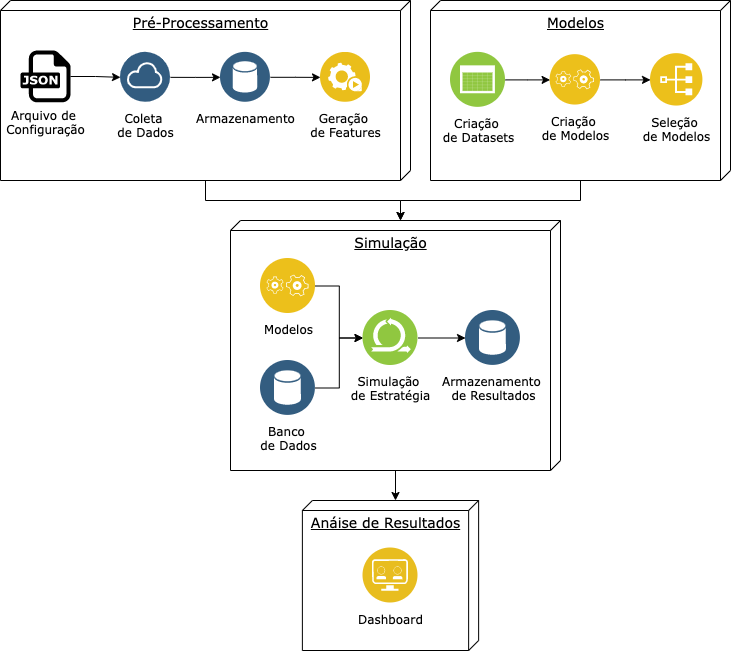
\includegraphics[scale=0.52]{resumo_projeto.png}
    \centering
    \caption{Estrutura do técnica do projeto}
    \label{fig:100}
\end{figure}

\paragraph{} Antes da execução do código principal, é necessário garantir que os modelos estão devidamente criados e acessíveis. Para isso, é importante a elaboração dos \textit{datasets} de cada ação a ser simulada, pois servem de entrada de dados para a criação e seleção de seus respectivos modelos. A biblioteca \textit{multiprocessing} foi utilizada para minimizar o tempo total gasto durante a criação dos modelos e da simulação das estratégias.

\paragraph{} Após a criação dos modelos, tem-se início a etapa de pré-processamento de dados, onde ocorre a leitura e interpretação do arquivo de configuração para se obter o número de estratégias a executar, além dos ativos envolvidos e seus respectivos intervalos de tempo. Uma vez verificado no banco os dados já existentes, faz-se um \textit{download} apenas dos dados necessários. Se houver alguma atualização, as \textit{features} de uso geral são recalculadas e armazenadas no banco a fim de servir de insumo para as estratégias que estarão por vir.

\paragraph{} Completada a etapa de pré-processamento, inicia-se a simulação das estratégias. O arquivo de configuração foi projetado para ser capaz de designar diversas estratégias de parâmetros distintos a uma mesma ordem de execução de programa, que ao final salva os resultados e as estatísticas no banco para posterior análise.

\paragraph{} Por fim, é possível visualizar os resultados de forma clara através de uma aplicação secundária responsável por criar um \textit{dashboard} interativo.

\paragraph{} Em relação às tecnologias utilizadas, a aplicação foi desenvolvida em \textit{Python} com o apoio das bibliotecas \textit{yfinance}, \textit{pandas}, \textit{numpy}, \textit{scikit-learn}, \textit{multiprocessing}, \textit{matplotlib} e \textit{dash}. Foi estruturado um banco de dados PostgreSQL \cite{postgresql} para armazenamento dos \textit{candlesticks} obtidos, das \textit{features} geradas e das estratégias simuladas. Também foi incorporado o uso de \textit{Docker} especificamente para a execução de estratégias sem a necessidade de configuração de ambiente.

\paragraph{} O \textbf{código fonte} do projeto pode ser encontrado em seu repositório online no Github \cite{project_github}.

\paragraph{} A Figura \ref{fig:444} mostra a sequência lógica de refinamento dos parâmetros de simulação. As Seções \ref{sub:max_op_days}, \ref{sub:operation_risk}, \ref{sub:risk_man} e \ref{sub:dynamic_rcc} tratam respectivamente do Período Máximo de Dias por Operação, da Margem de Risco, do Coeficiente de Risco-Capital (RCC) e da Constante de Ganho Proporcional (K). Nota-se que o valor de saída de um parâmetro é utilizado durante o refinamento parâmetro do seguinte. Com exceção do Período Máximo de Dias por Operação, que utilizou o intervalo de 2016 a 2018, os outros parâmetros foram refinados a partir de simulações no intervalo de janeiro de 2019 a março de 2020, denominado intervalo de refinamento de parâmetros de estratégia. Já o resultado da simulação final, disponível na Seção \ref{cap4}, utiliza o intervalo de abril de 2020 a dezembro de 2021, não havendo assim sobreposição.

\begin{figure}[!htb]
    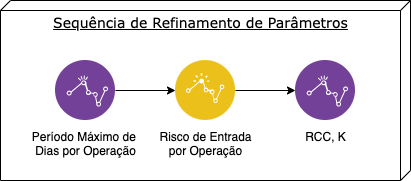
\includegraphics[scale=0.65]{otimizacao_de_parametros.png}
    \centering
    \caption{Sequência de Refinamento de Parâmetros}
    \label{fig:444}
\end{figure}

\paragraph{} A Tabela \ref{tab:5} lista todos os 71 ativos escolhidos para simulação no escopo deste trabalho. Os critérios de escolha envolveram as seguintes preferências: diversidade de segmentos; disponibilidade da série temporal de dados a partir de 2013; e presença na composição do iBovespa em qualquer data. Além disso, o alto número de ativos foi escolhido para aumentar a diversidade de padrões nos movimentos dos preções, o que pode trazer mais clareza quanto a qualidade média dos modelos durante análise dos resultados.

{\small
\begin{longtable}[c]{ccc}
    \caption{Ações Escolhidas (71) \\
    \label{tab:5}} \\

    Companhia & \textit{Ticker} & Segmento Econômico \\
    \hline
    \endfirsthead


    \multicolumn{3}{c}{Continuação da Tabela \ref{tab:5}} \\
    \hline
    Companhia & \textit{Ticker} & Segmento Econômico \\
    \hline
    \endhead

    \endfoot

    \hline
    \multicolumn{3}{c}{Fim da Tabela \ref{tab:5}} \\
    \endlastfoot

    AMBEV S/A & ABEV3 & Cervejas e Refrigerantes \\
    ALPARGATAS & ALPA4 & Calçados \\
    AMERICANAS SA & AMER3 & Produtos Diversos \\
    B3 & B3SA3 & Serviços Financeiros Diversos \\
    BRASIL & BBAS3 & Bancos \\
    BRADESCO & BBDC3 & Bancos \\
    BRADESCO & BBDC4 & Bancos \\
    BB SEGURIDADE & BBSE3 & Seguradoras \\
    MINERVA & BEEF3 & Carnes e Derivados \\
    BANCO PAN & BPAN4 & Bancos \\
    BRADESPAR & BRAP4 & Minerais Metálicos \\
    BRF SA & BRFS3 & Carnes e Derivados \\
    BRASKEM & BRKM5 & Petroquímicos \\
    BR MALLS PAR & BRML3 & Exploração de Imóveis \\
    CCR SA & CCRO3 & Exploração de Rodovias \\
    CIELO & CIEL3 & Serviços Financeiros Diversos \\
    CEMIG & CMIG4 & Energia Elétrica \\
    COGNA ON & COGN3 & Serviços Educacionais \\
    CPFL ENERGIA & CPFE3 & Energia Elétrica \\
    COPEL & CPLE6 & Energia Elétrica \\
    COSAN & CSAN3 & Exploração, Refino e Distribuição \\
    SID NACIONAL & CSNA3 & Siderurgia \\
    CVC BRASIL & CVCB3 & Viagens e Turismo \\
    CYRELA REALT & CYRE3 & Incorporações \\
    DEXCO SA & DXCO3 & Madeiras \\
    ECORODOVIAS & ECOR3 & Exploração de Rodovias \\
    ENGIE BRASIL & EGIE3 & Energia Elétrica \\
    ELETROBRAS & ELET3 & Energia Elétrica \\
    ELETROBRAS & ELET6 & Energia Elétrica \\
    EMBRAER & EMBR3 & Material Aeronáutico e de Defesa \\
    ENERGIAS BR & ENBR3 & Energia Elétrica \\
    ENEVA & ENEV3 & Energia Elétrica \\
    ENERGISA & ENGI11 & Energia Elétrica \\
    EQUATORIAL & EQTL3 & Energia Elétrica \\
    EZTEC & EZTC3 & Incorporações \\
    FLEURY & FLRY3 & Serviços Médicos \\
    GERDAU & GGBR4 & Siderurgia \\
    GERDAU MET & GOAU4 & Siderurgia \\
    GOL & GOLL4 & Transporte Aéreo \\
    HYPERA & HYPE3 & Medicamentos e Outros Produtos \\
    ITAUSA & ITSA4 & Bancos \\
    ITAU UNIBANCO & ITUB4 & Bancos \\
    JBS & JBSS3 & Carnes e Derivados \\
    JHSF PART & JHSF3 & Incorporações \\
    LOJAS AMERICANAS & LAME4 & Produtos Diversos \\
    LOCAMERICA & LCAM3 & Aluguel de carros \\
    LOJAS RENNER & LREN3 & Tecidos, Vestuário e Calçados \\
    MAGAZINE LUIZA & MGLU3 & Eletrodomésticos \\
    MARFRIG & MRFG3 & Carnes e Derivados \\
    MRV & MRVE3 & Incorporações \\
    MULTIPLAN & MULT3 & Exploração de Imóveis \\
    PETROBRAS & PETR3 & Exploração, Refino e Distribuição \\
    PETROBRAS & PETR4 & Exploração, Refino e Distribuição \\
    POSITIVO TEC & POSI3 & Computadores e Equipamentos \\
    PETRORIO & PRIO3 & Exploração, Refino e Distribuição \\
    QUALICORP & QUAL3 & Serviços Médicos \\
    RAIADROGASIL & RADL3 & Medicamentos e Outros Produtos \\
    LOCALIZA & RENT3 & Aluguel de carros \\
    SANTANDER BR & SANB11 & Bancos \\
    SABESP & SBSP3 & Água e Saneamento \\
    SUL AMERICA & SULA11 & Seguradoras \\
    TAESA & TAEE11 & Energia Elétrica \\
    TIM BRASIL & TIMS3 & Telecomunicações \\
    TOTVS & TOTS3 & Programas e Serviços \\
    ULTRAPAR & UGPA3 & Exploração, Refino e Distribuição \\
    USIMINAS & USIM5 & Siderurgia \\
    VALE & VALE3 & Minerais Metálicos \\
    VIA SA & VIIA3 & Eletrodomésticos \\
    TELEF BRASIL & VIVT3 & Telecomunicações \\
    WEG & WEGE3 & Motores, Compressores e Outros \\
    YDUQS PART & YDUQ3 & Serviços Educacionais \\


\end{longtable}}



\FloatBarrier
\section{Pré-Processamento}

\FloatBarrier
\subsection{Arquivo de Configuração}
\label{sub:conf_file}

\paragraph{} O Arquivo de Configuração é um arquivo no formato JSON responsável por configurar detalhadamente cada parâmetro da sequência de estratégias que se deseja executar. Uma ordem de execução do programa pode conter diversas simulações de estratégias, que são configuradas neste Arquivo. A Figura \ref{fig:101} mostra sua estrutura.

\begin{figure}[!htb]
    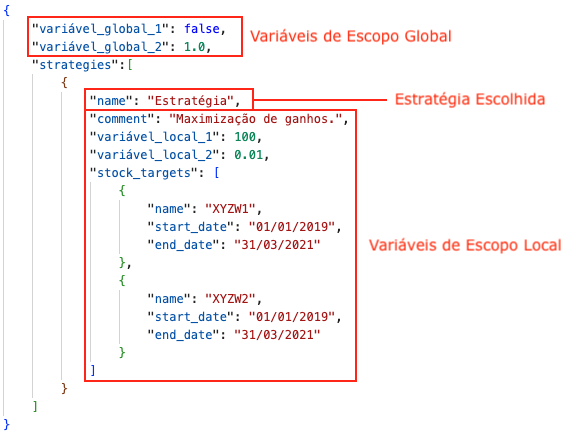
\includegraphics[scale=0.50]{config_file_estrutura.png}
    \centering
    \caption{Estrutura do Arquivo de Configuração}
    \label{fig:101}
\end{figure}

\paragraph{} Nota-se que no topo são listados os parâmetros de uso geral, ou variáveis de escopo global, cujos valores precedem quaisquer outros listados na sequência, em caso de sobreposição. Em seguida abre-se o vetor de tipos de estratégias, onde o campo \textit{name} representa o nome da classe selecionada, sendo este o elemento que conecta o usuário ao tipo de estratégia desejada. Ressalta-se que este trabalho compreende apenas um tipo de estratégia, embora o arquivo permita a leitura de qualquer nome. Na sequência, são configurados os parâmetros internos da estratégia. A Tabela \ref{tab:3} da Seção \ref{sub:params_list} descreve todos os parâmetros disponíveis.

\paragraph{} Para se criar mais de um perfil de simulação, isto é, uma única execução do programa executar várias simulações via multiprocessamento, é necessário modificar o Arquivo conforme a Figura \ref{fig:102}. Automaticamente, o código interpreta que existe mais de uma simulação a executar, com todos os parâmetros em comum exceto aqueles em formato de listas. Caso haja mais de um parâmetro no formato de lista, seus comprimentos precisam ser iguais. No caso da Figura \ref{fig:102}, a primeira simulação utilizará os valores (100, 0.01) para o par (variável\_local\_1, variável\_local\_2), a segunda utilizará (200, 0.02) e assim sucessivamente.

\begin{figure}[!htb]
    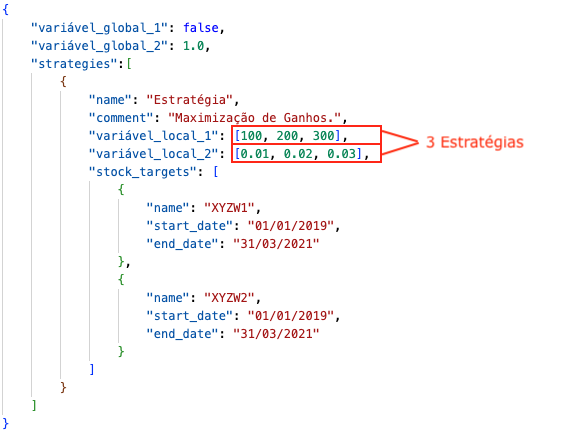
\includegraphics[scale=0.50]{config_file_mult_exec.png}
    \centering
    \caption{Arquivo de Configuração para Execuções Múltiplas}
    \label{fig:102}
\end{figure}



\FloatBarrier
\subsection{Coleta de Dados}
\label{coleta_de_dados}

\paragraph{} A Coleta de Dados ocorre através da biblioteca \textit{open-source} \textit{yfinance} \cite{yfinance}, uma ferramenta não oficial que transmite dados obtidos através de APIs públicas da plataforma \textit{Yahoo! Finance} \cite{yahoo_finance}, um subsistema da rede \textit{Yahoo!}.

\paragraph{} A escolha desta biblioteca como fonte primária de dados se deve principalmente pela facilidade de uso associada à ausência de custos. Contudo, alguns testes e verificações com outras fontes de dados evidenciaram destantagens relevantes, porém não impeditivas para uso. São elas:

\begin{itemize}
    \item Os valores de proventos que a biblioteca disponibiliza não são consistentes com as declarações dos sites das próprias companhias, portanto não podem ser utilizados por este projeto. Testes internos confirmaram a presença de diversos proventos corretamente apresentados e ajustados pelos respectivos desdobramentos acumulados. O problema é que os mesmos estavam misturados com alguns \textit{outliers} inexistentes na realidade, o suficiente para questionar o uso em escala (\textit{i.e.}, para vários ativos sem verificação individual). O Apêndice \ref{ApendiceA} evidencia os problemas encontrados em mais detalhes.

    \item Até onde se pode verificar, os volumes de negociação disponibilizados coincidem em valores relativos com os volumes da plataforma \textit{TradingView} \cite{tradingview}, não tendo sido encontrada evidência do contrário. Em outras palavras, a variação percentual de volume entre dois pregões de um mesmo ativo é igual em ambas as plataformas.

    \item \textit{Candlesticks} de janelas temporais inferiores à diária (\textit{intraday}) são disponibilizados, porém o limite de busca de 730 dias inviabiliza seu uso.
\end{itemize}

% Aqui fala da criação de candles semanais
% \paragraph{} Os dados obtidos são \textit{candlesticks} diários (OHLCV). Com a mesma facilidade, é possível adquirir janelas de tempo semanais, no entanto para evitar potenciais problemas de consistência de dados, as mesmas são calculadas internamente a partir da janela diária via comandos SQL\footnote{\textit{Structured Query Language}: Linguagem usada para administrar bancos de dados relacionais.}.

\paragraph{} Apenas os dados não existentes no banco são baixados via \textit{yfinance}. Para isso, um \textit{trigger}\footnote{Procedimento armazenado em um banco de dados que é chamado automaticamente sempre que ocorre um evento determinado.} é acoplado às tabelas de \textit{candlesticks} e acionado sempre que operações de \textit{insert}, \textit{update}, \textit{delete} e \textit{truncate} são realizadas. Quando ativado, ele chama uma função responsável por atualizar a tabela de \textit{status}, que registra o intervalo de tempo representado nas tabelas de \textit{candlesticks} para cada \textit{ticker} envolvido. Deve-se ressaltar que os devidos cuidados foram tomados para evitar buracos entre intervalos de tempo não adjacentes. Portanto, apenas uma consulta à tabela de \textit{status} é executada para se verificar a necessidade de \textit{download} de novos dados.



\FloatBarrier
\subsection{Armazenamento de Dados}

\paragraph{} O Armazenamento de Dados é realizado por um banco de dados \textit{PostgreSQL}, criado com o objetivo de salvar: os resultados das simulações; as \textit{features} de uso geral; e os \textit{candlesticks} obtidos. As vantagens de um banco de dados em relação a um arquivo CSV ou a uma planilha de Excel dispensam comentários. Contudo, quanto ao escopo deste trabalho, pode-se mencionar os seguintes pontos:

\begin{itemize}
    \item Fácil acesso aos resultados das simulações de forma estruturada e consistente, recurso este utilizado pela aplicação que gera o \textit{dashboard}.
    \item Economia de processamento devido ao armazenamento das \textit{features} de uso geral, uma vez que estratégias simuladas não necessitam recalculá-las a cada execução.
    \item Independência da plataforma \textit{Yahoo! Finance} para o caso de não continuidade dos dados ou qualquer alteração repentida.
    \item Diminuição do tráfego na rede pela persistência dos \textit{candlesticks} já obtidos.
\end{itemize}

% Aqui fala da criação de candles semanais
% \paragraph{} Os \textit{candlesticks} semanais são calculados via \textit{query} SQL para garantir a consistência dos dados, já que a possibilidade de inconsistência se fez presente entre dados \textit{intraday} e diários, conforme mencionado na Seção \ref{coleta_de_dados}.

\paragraph{} A figura \ref{fig:103} mostra o ERD\footnote{\textit{Entity-Relationship Diagram}. Em português: Diagrama de Entidade Relacionamento.} do banco de dados. Os \textit{scripts} de criação e população inicial, bem como as \textit{constraints} envolvidas podem ser encontrados em \cite{github_db_schema}.

\begin{landscape}

\begin{figure}[!htb]
    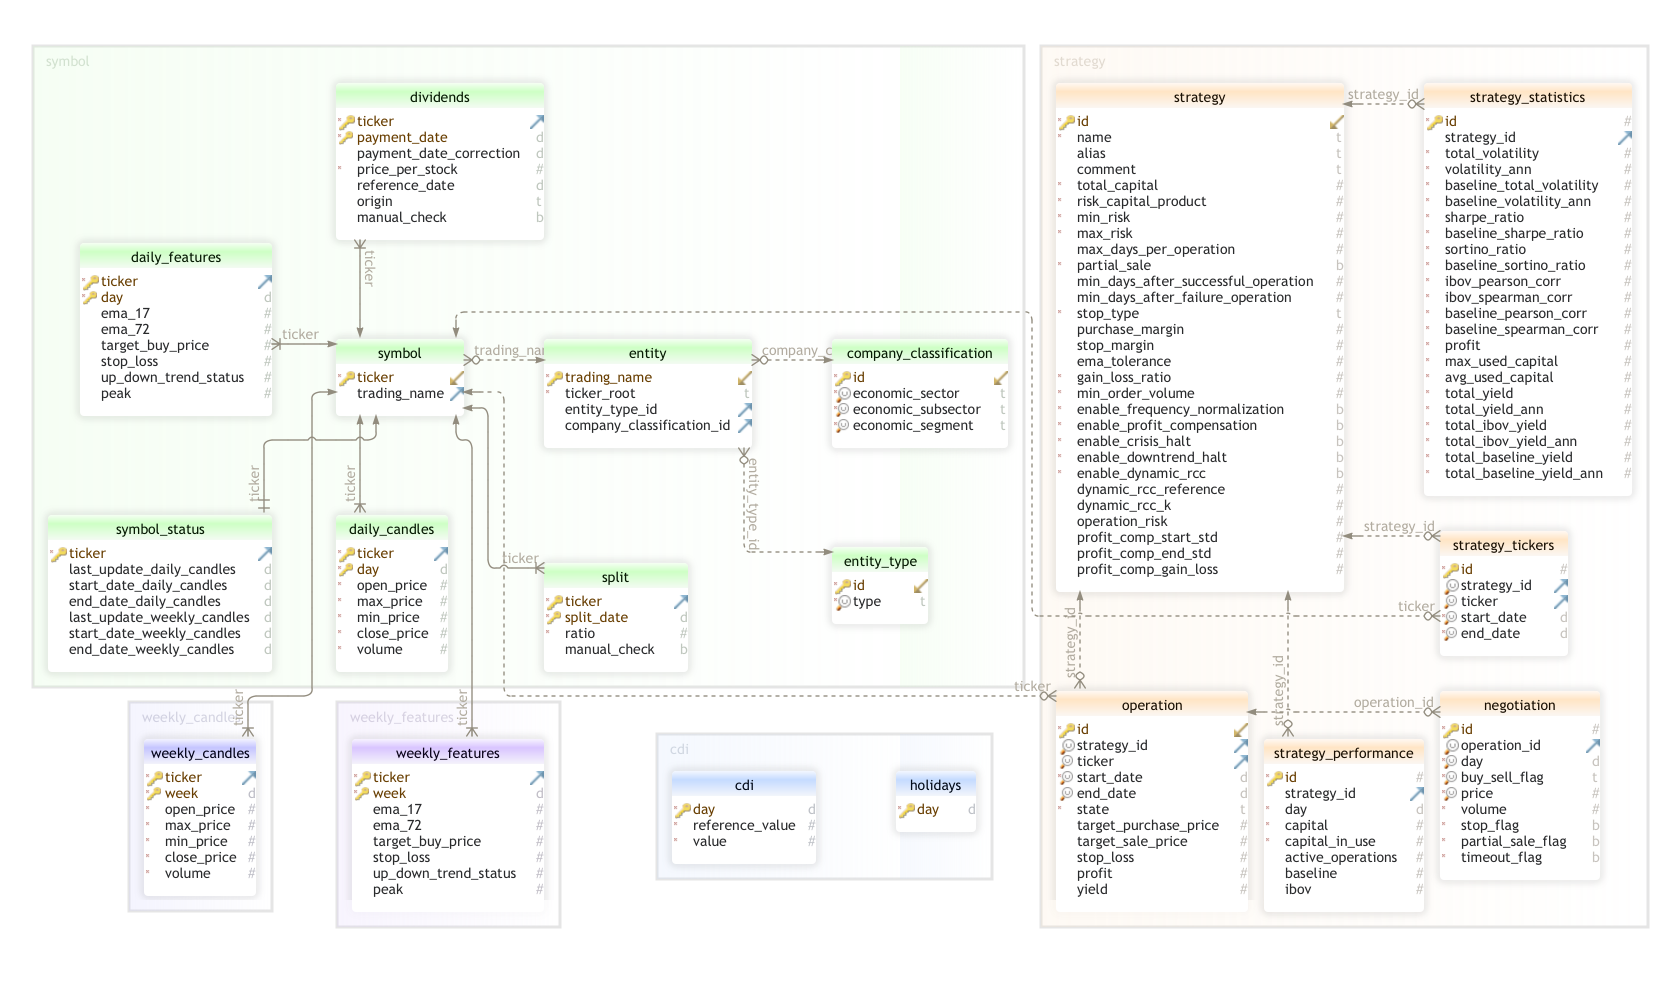
\includegraphics[scale=0.40]{ERD.png}
    \centering
    \caption{ERD do Banco de Dados}
    \label{fig:103}
\end{figure}

\end{landscape}

% \begin{figure}[!htb]
%     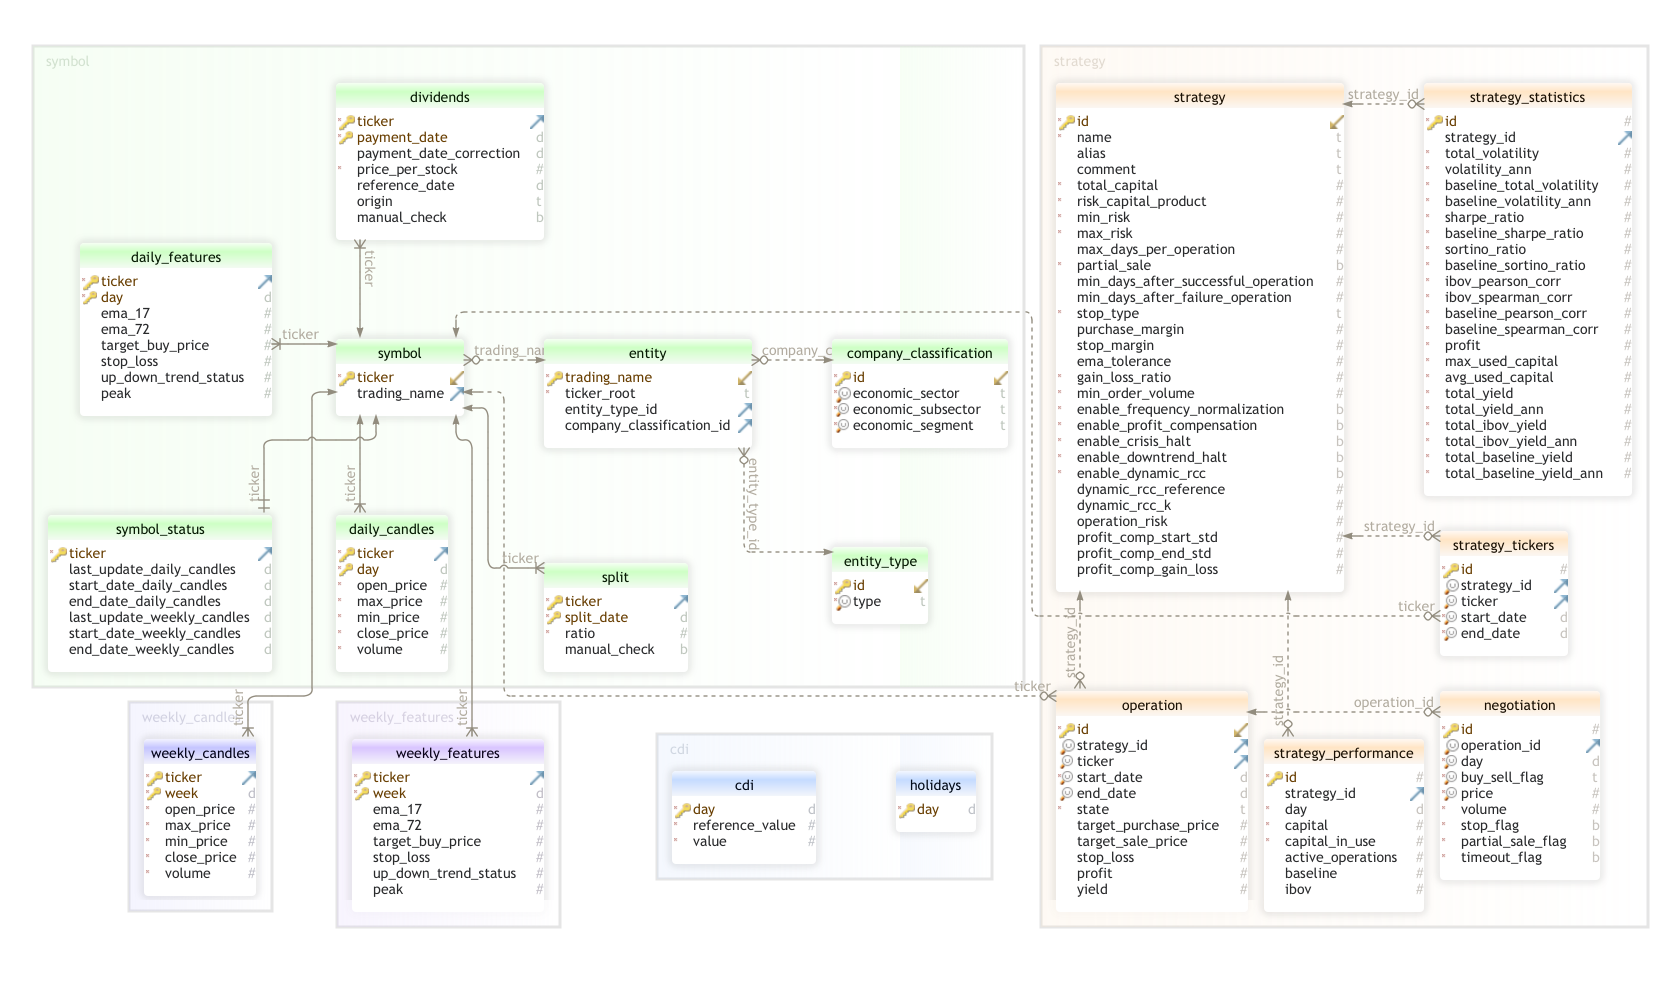
\includegraphics[scale=0.10]{ERD.png}
%     \centering
%     \caption{ERD do Banco de Dados}
%     \label{fig:103}
% \end{figure}



\FloatBarrier
\subsection{Geração de \textit{Features} de Uso Geral}
\label{sub:features}

\paragraph{} As \textit{Features} de Uso Geral são características derivadas dos \textit{candlesticks} que podem auxiliar qualquer decisão interna de uma estratégia. Mais especificamente, esta Seção aborda as \textit{features} Risco Mínimo e Rísco Máximo, que possuem duas funções principais: auxiliar no processo de escolha do preços de compra, dos \textit{stop loss} e dos preços alvo através do parâmetro Margem de Risco; e auxiliar os modelos de ML a decidirem o momento apropriado de compra dos ativos, com base nos valores dos preços encontrados.

\paragraph{} Devido à natureza genérica das \textit{features}, que podem ser utilizadas por diversas estratégias, são calculadas antes do início das simulações e somente quando há necessidade, ou seja, quando os \textit{candlesticks} são inseridos pela primeira vez no banco ou quando são atualizados. Ao final dos cálculos, são armazenadas nas tabelas de \textit{features} para posteriores consultas durante as simulações.

\paragraph{} O fato dos cálculos envolverem uma análise de dados do passado, é necessário garantir que as \textit{features} geradas estejam sempre apontadas para um intervalo de tempo anterior ao dia no qual elas serão consumidas. Do contrário, um erro de não-causalidade poderia surgir, corrompendo a performance das simulações. Analogamente, durante a geração dos modelos (Seção \ref{sub:models_gen}) também é necessario se garantir que o período de treinamento é anterior ao período de teste, diretamente via a configuração das datas limites de cada período e indiretamente via remoção de datas cuja \textit{features} possuem efeito memória, evitando assim que qualquer informação esteja presente simultaneamente dos dados de treinamento e de teste.

\paragraph{} Antes de prosseguir, é necessário contextualizar o termo risco de entrada em uma operação, às vezes simplesmente chamado de risco. Este é caracterizado pela diferença percentual no qual o \textit{stop loss} é colocado em relação ao do preço de compra. Por exemplo, se uma operação tem um preço de compra de R\$10,00 e o \textit{stop loss} é posicionado em R\$9,00, diz-se o risco da operação é de 10\%. A escolha do risco também determina o valor do preço alvo da operação, pois o mesmo é definido como 3 vezes a magnitude do risco escolhido, percentualmente e acima do preço de compra (ver Seção \ref{sub:estrutura}). Assim, no exemplo anterior, o preço alvo estaria situado em R\$13,00. Este assunto será novamente abordado na Seção \ref{sub:estrutura}, no entanto fez-se necessária uma antecipação pois esta terminologia é amplamente utilizada ao longo deste trabalho.

\paragraph{} As \textit{features} de Uso Geral utilizadas são:

\begin{itemize}

    \item \textbf{Risco Mínimo} \\ \\
    O Risco Mínimo é uma \textit{feature} de suporte à escolha do risco de entrada em uma operação, não sendo assim consumido diretamente pelo modelo de ML, mas sim indiretamente. A fórmula é composta por uma parcela fixa somada a uma parcela variável, conforme mostrado pela Equação \ref{eq:30}.

    \begin{equation} \label{eq:30}
        Risk_{min} = Risk_{min_f} + Risk_{min_v}
    \end{equation}

    Seja \begin{math} P_{\Delta} \end{math} a diferença entre o preço máximo e mínimo de um \textit{candle} (Equação \ref{eq:31}), pode-se definir \begin{math} Risk_{min_f} \end{math} como o valor mínimo de risco necessário para superar as oscilações diárias dos preços médios dos últimos 20 dias úteis (Equações \ref{eq:22} e \ref{eq:32}). Nota-se que \begin{math} \sigma_{P_{\Delta}} \end{math} é o desvio padrão relativo aos últimos 20 dias úteis.

    \begin{equation} \label{eq:31}
        P_{\Delta} = P_{high} - P_{low}
    \end{equation}

    \begin{equation} \label{eq:22}
        P_{mid} = \dfrac{P_{open} + P_{close}}{2}
    \end{equation}

    \begin{equation} \label{eq:32}
        Risk_{min_f} = \dfrac{ \sigma_{P_{\Delta}} }{ P_{mid} }
    \end{equation}

    A parcela variável \begin{math} Risk_{min_v} \end{math} está associada à tendência de queda de preço no curto prazo. Seu cálculo é realizado a partir da derivada de preços médios ajustada por um filtro digital IIR passa-baixas \cite{haykin2007signals} (Equações \ref{eq:23}, \ref{eq:24} e \ref{eq:33}), onde \begin{math} \alpha \end{math} é o coeficiente de amortecimento. Observa-se que a derivada do preço médio foi normalizada para permitir que a tendência independa do valor absoluto do preço, tratando-se apenas de uma variação percentual. O sinal negativo na Equação \ref{eq:33} indica que quanto maior a tendência de queda, maior precisa ser o risco associado.

    \begin{equation} \label{eq:23}
        \dot{P_{mid(i)}} = \dfrac{ P_{mid(i)} - P_{mid(i-1)} }{ \dfrac{1}{2}(P_{mid(i)} + P_{mid(i-1)}) }
    \end{equation}

    \begin{equation} \label{eq:24}
        \dot{P_{mid\_LPF(i)}} = \alpha \dot{P_{mid(i)}} + (1 - \alpha) \dot{P_{mid\_LPF(i-1)}},  \quad \textrm{onde} \quad 0 \le \alpha \le 1
    \end{equation}

    \begin{equation} \label{eq:33}
        Risk_{min_v} = max(-\dot{P_{mid\_LPF(i)}}, 0)
    \end{equation}

    Foi utilizado \begin{math} \alpha = 0.30 \end{math}, uma vez que neste caso é mais interessante uma resposta rápida a um baixo ruído.

    Por fim, adicionou-se um segundo filtro de passa-baixas de \begin{math} \alpha = 0.10 \end{math} apenas aos movimentos de descida dos valores de \begin{math} Risk_{min} \end{math} com o objetivo de aumentar a cautela durante momentos mais turbulentos do mercado.

    As Figuras \ref{fig:400} e \ref{fig:105} e mostram os resultados do algoritmo para dois papéis de comportamentos distintos: MGLU3 representando um companhia com foco em alto crescimento, portanto mais volátil; e ABEV3 representando uma companhia já bem consolidada no mercado, portanto menos volátil.

    \begin{figure}[!htb]
        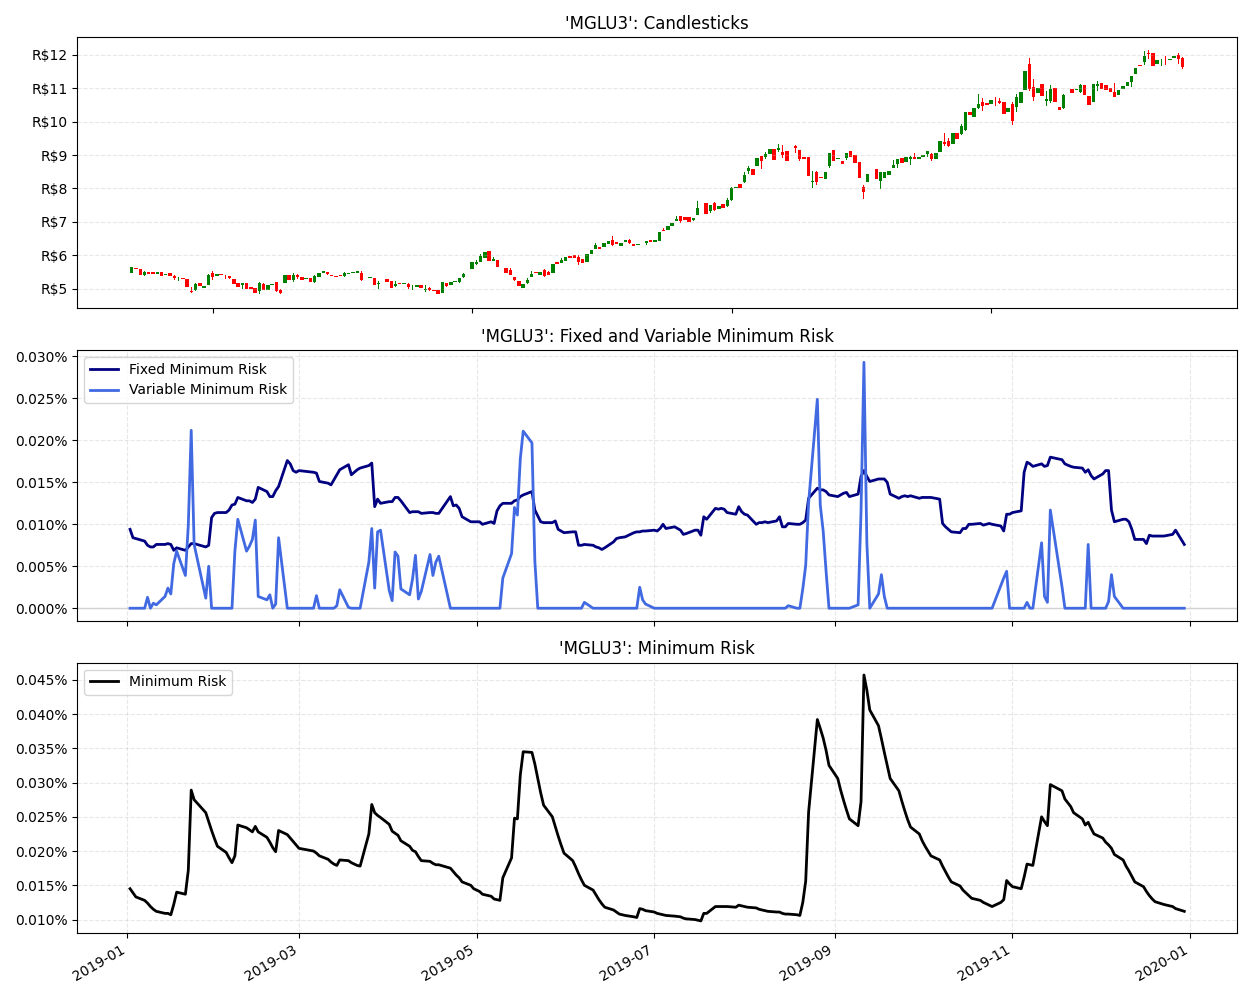
\includegraphics[scale=0.41]{min_risk_mglu3.png}
        \centering
        \caption{MGLU3 - Risco Mínimo (01/01/2019 a 31/12/2019)}
        \label{fig:400}
    \end{figure}

    \begin{figure}[!htb]
        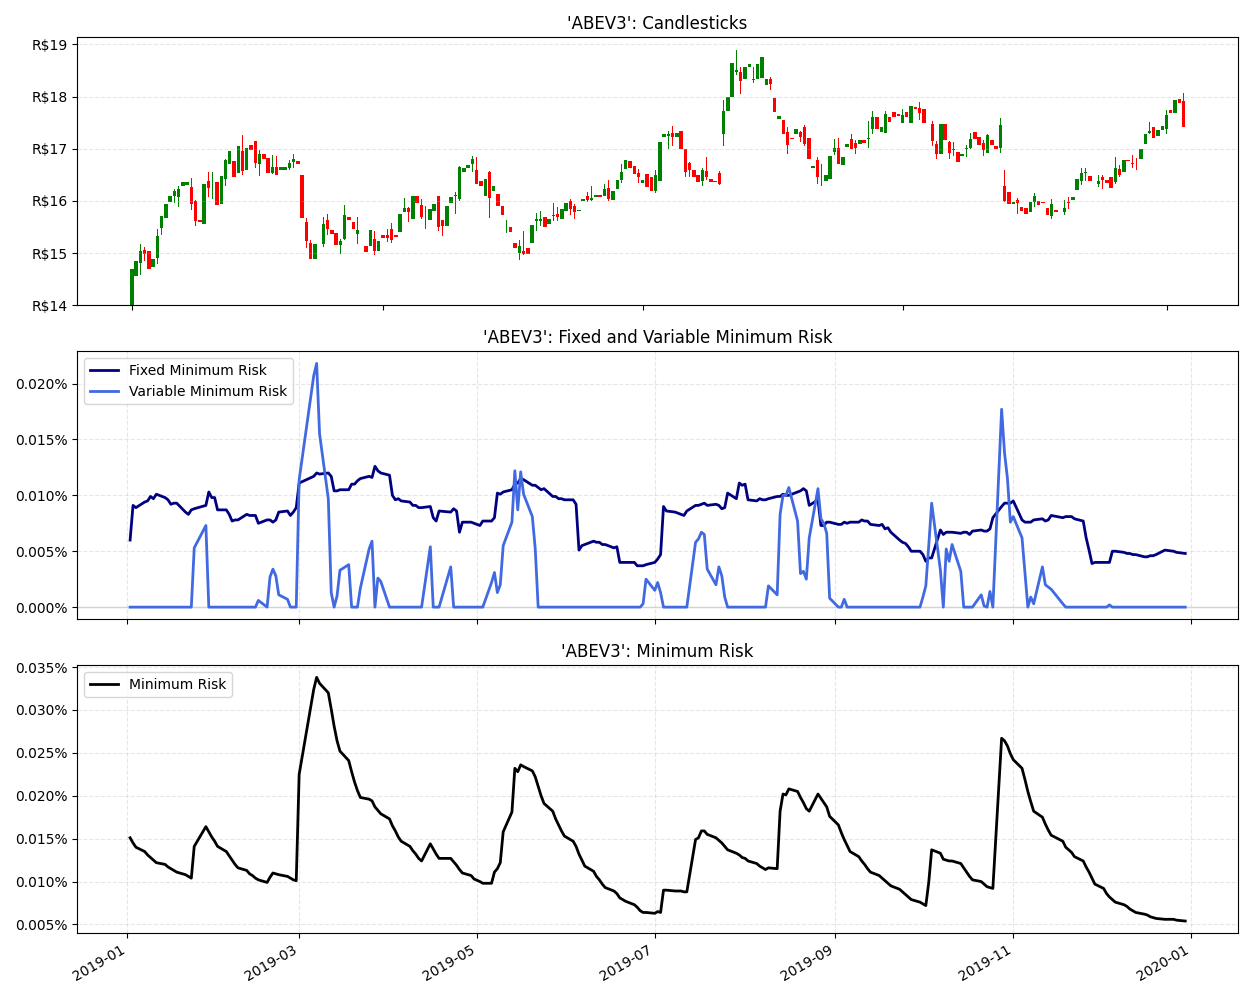
\includegraphics[scale=0.41]{min_risk_abev3.png}
        \centering
        \caption{ABEV3 - Risco Mínimo (01/01/2019 a 31/12/2019)}
        \label{fig:105}
    \end{figure}


    \item \textbf{Risco Máximo} \\ \\
    O Risco Máximo é uma \textit{feature} de suporte à escolha do risco de entrada em uma operação, não sendo assim consumido diretamente pelo modelo de ML, mas sim indiretamente. A ideia central está na análise estatística das subidas de preços entre os últimos picos identificados dentro do intervalo de 80 dias úteis.

    Para se iniciar o cálculo, primeiro é necessário a criação de um algoritmo de identificação de picos, conforme mostrado pela Figura \ref{fig:106}. O método usa uma janela móvel de \begin{math} W \end{math} \textit{candles} que corre dia após dia até a data corrente e atribui 1 voto de máximo e 1 voto de mínimo aos preços de máximo e aos preços de mínimo encontrados na janela, respectivamente. Segundo André Moraes \cite{moraes2007se}, uma janela de \begin{math} W = 17 \end{math} \textit{candles} é uma boa escolha para identifição de picos no gráfico diário, mas com o objetivo de se analisar a tendência de mercado. Optou-se por uma janela de \begin{math} W = 5 \end{math} \textit{candles} para aumentar a densidade de picos encontrados, facilitando assim as análises estatísticas seguintes.

    Em todos os passos, o primeiro e o último \textit{candle} da janela nunca recebem votos devido à falta de um \textit{candle} adjacente. São elegíveis à picos apenas os \textit{candles} que obtiveram um mínimo de \begin{math}  floor(W / 2) = 2 \end{math} votos. Ao final, garante-se a alternância entre máximos e mínimos locais através da remoção de picos consecutivos de um mesmo tipo.

    \begin{figure}[!htb]
        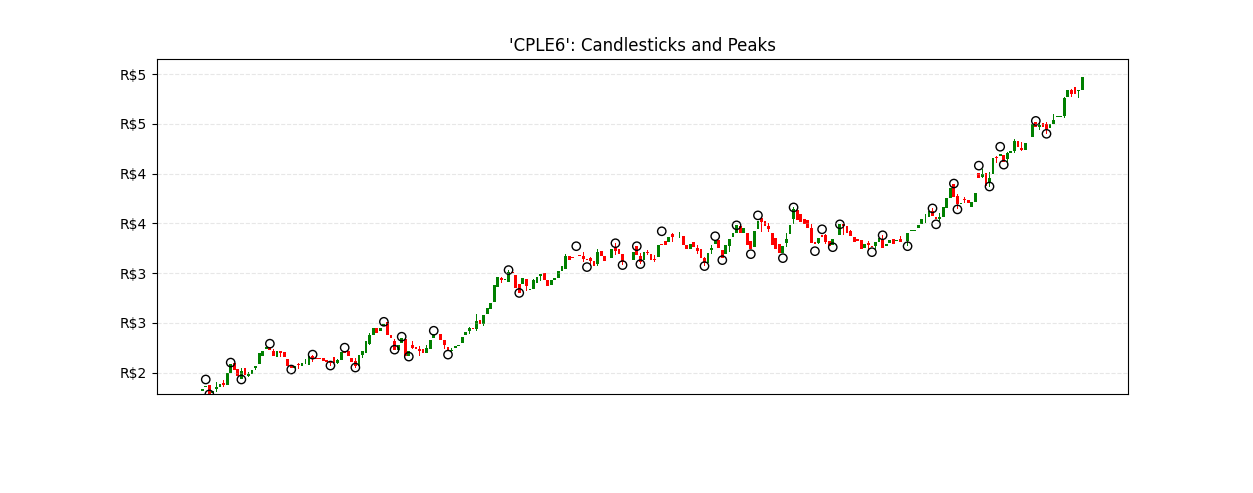
\includegraphics[scale=0.47]{peaks_cple6_w_5.png}
        \centering
        \caption{CPLE6 - Algoritmo de identificação de picos (01/01/2019 a 31/12/2019)}
        \label{fig:106}
    \end{figure}

    Depois da identificação de picos, extraem-se as \begin{math} n \end{math} subidas de preços de cada mínimo para o máximo consecutivo no período designado, normalizados pelo pico de mínimo (Figura \ref{fig:107} e Equação \ref{eq:40}). Por fim, o Risco máximo é obtido pelo cálculo da média \begin{math} \overline{C_{(i)}} \end{math} com um filtro digital IIR passa-baixas (Equações \ref{eq:41} e \ref{eq:42}).

    \begin{figure}[!htb]
        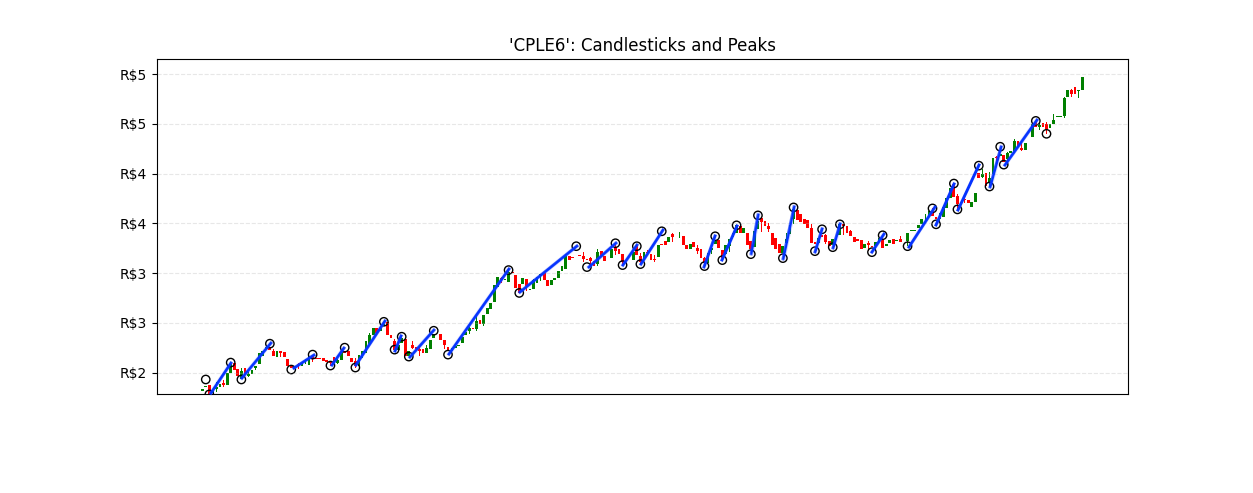
\includegraphics[scale=0.47]{peaks_with_marks_cple6_w_5.png}
        \centering
        \caption{CPLE6 - Subidas de preços entre picos (01/01/2019 a 31/12/2019)}
        \label{fig:107}
    \end{figure}

    \begin{equation} \label{eq:40}
        c_k = (P_{max(k)} - P_{min(k)}) / P_{min(k)}, \quad \textrm{onde } 0 < k \le n
    \end{equation}

    \begin{equation} \label{eq:41}
        \overline{C_{(i)}} = \dfrac{1}{n} \sum_{k=1}^{n} c_k
    \end{equation}

    \begin{equation} \label{eq:42}
        Risk_{max(i)} = \alpha \overline{C_{(i)}} + (1 - \alpha) Risk_{max(i-1)}
    \end{equation}

    \begin{equation} \label{eq:43}
        \overline{C_{LPF(i)}} = \alpha \overline{C_{(i)}} + (1 - \alpha) \overline{C_{(i-1)}}
    \end{equation}

    \begin{equation} \label{eq:44}
        Risk_{max(i)} = \dfrac{\overline{C_{LPF(i)}} - 0.5 \sigma_{C}}{G}
    \end{equation}

    Foi utilizado \begin{math} \alpha = 0.50 \end{math}.

    As Figuras \ref{fig:108} e \ref{fig:270} mostram o Risco Máximo para os ativos MGLU3 e ABEV3, respectivamente.

    \begin{figure}[!htb]
        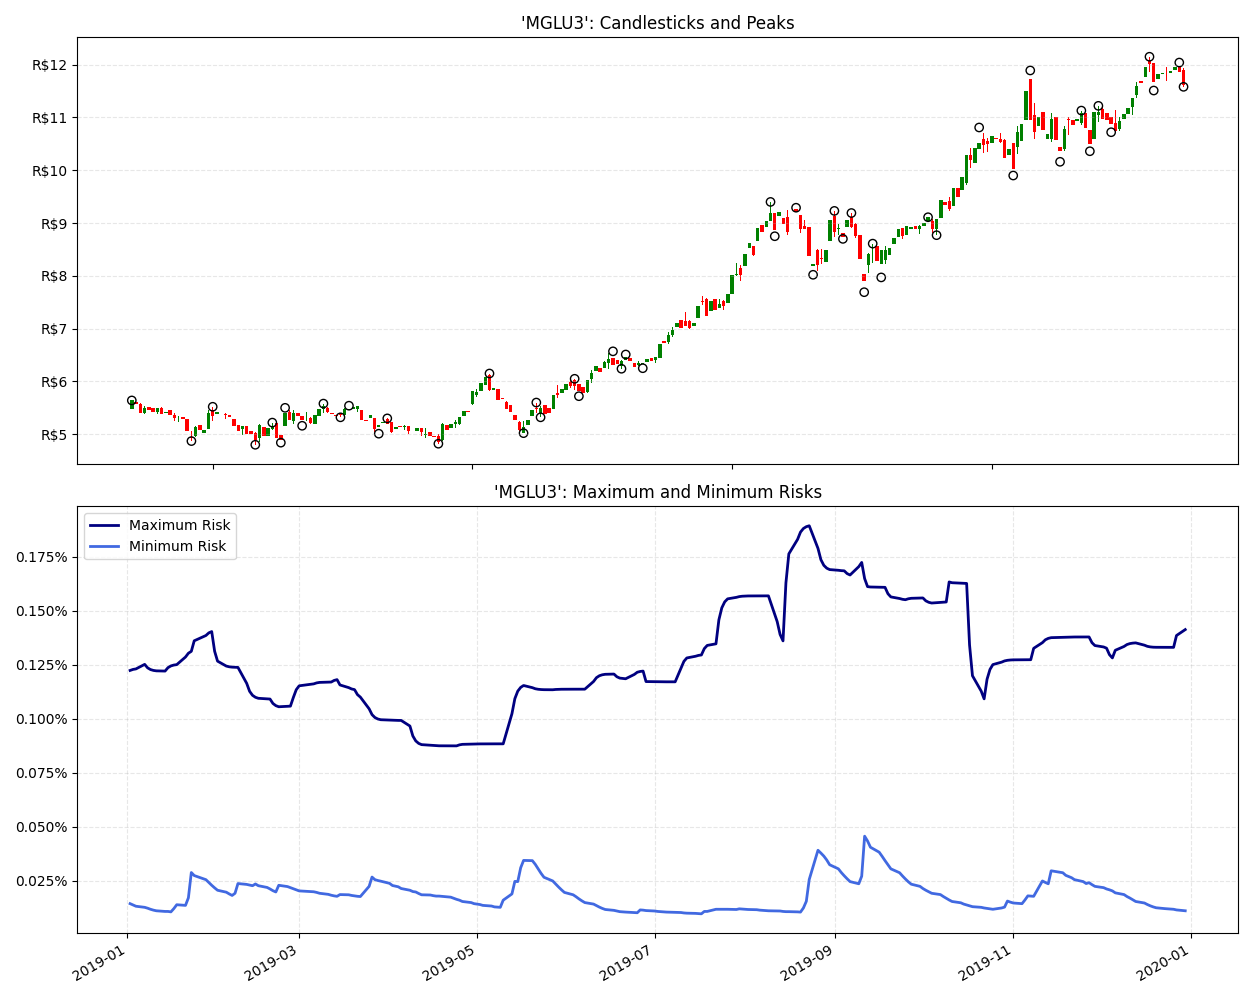
\includegraphics[scale=0.41]{max_risk_mglu3.png}
        \centering
        \caption{MGLU3 - Riscos Máximo e Mínimo (01/01/2019 a 31/12/2019)}
        \label{fig:108}
    \end{figure}

    \begin{figure}[!htb]
        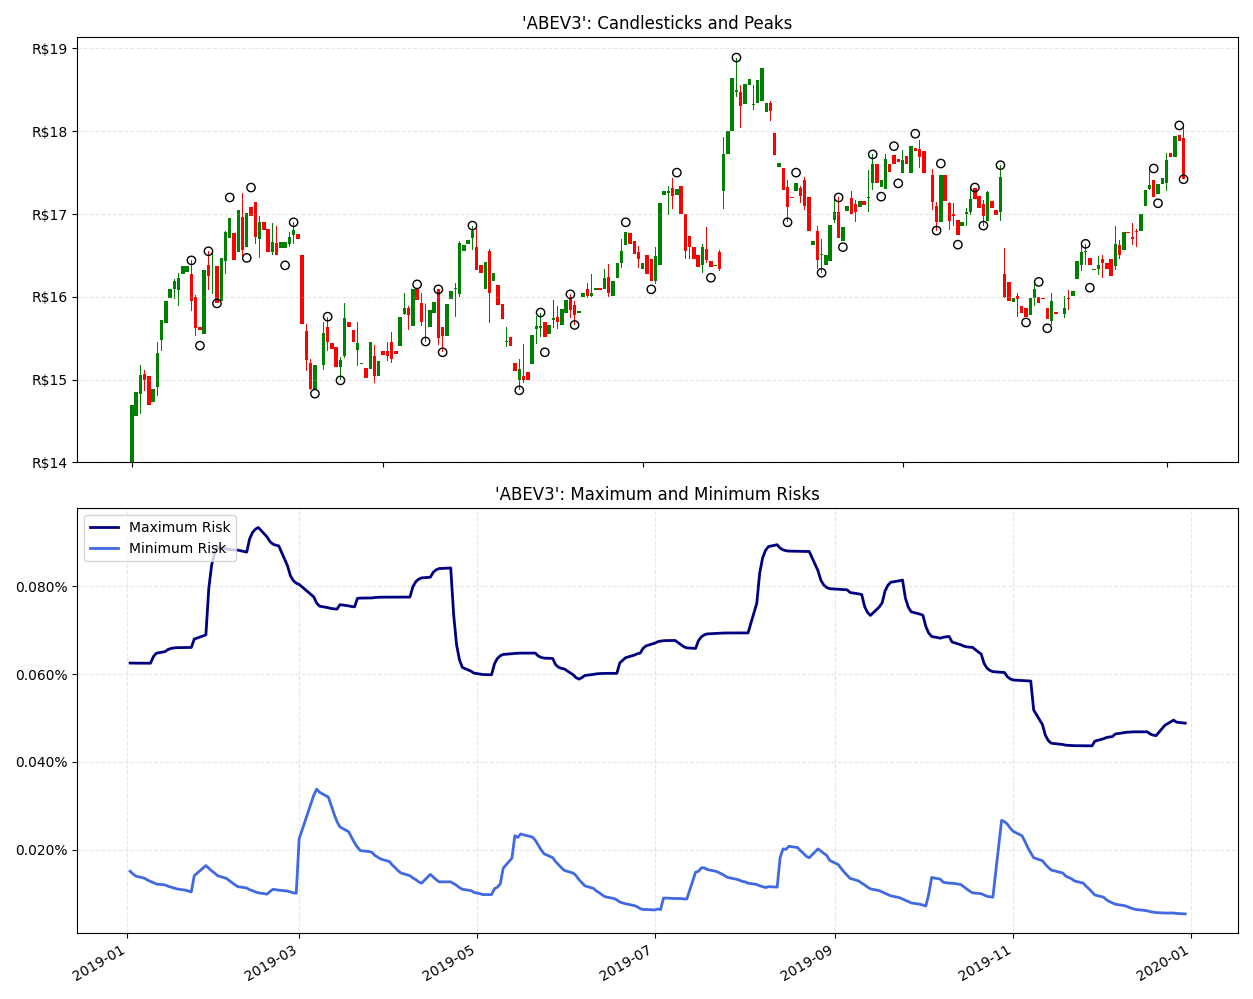
\includegraphics[scale=0.41]{max_risk_abev3.png}
        \centering
        \caption{ABEV3 - Riscos Máximo e Mínimo (01/01/2019 a 31/12/2019)}
        \label{fig:270}
    \end{figure}

\end{itemize}




\FloatBarrier
\section{Modelos de Aprendizado Supervisionado}
\label{sub:super_models}


\FloatBarrier
\subsection{Visão Geral}

\paragraph{} Conforme mostrado na Seção \ref{sub:ml_models_study}, a literatura aponta para o uso de modelos dos tipos ANN, SVM e lógica \textit{Fuzzy}. No entanto, escolheu-se \textit{Random Forests} devido à sua baixa tendência de \textit{overfitting} e à ausência de necessidade de escalamento das \textit{features} consumidas. Apesar de ser um modelo com várias possibilidades de hiperparâmetros a serem ajustados, a prática mostra que poucos são aqueles que realmente trazem uma melhora de performance significativa, uma vez que uma RF que tenha atingido um número alto o suficiente de árvores.

\paragraph{} A partir de \textit{datasets} previamente populados, modelos são gerados para cada ação a cada intervalo de 3 meses de simulação devido aos uso de WFA. Um critério particular de performance foi criado para ranquear os melhores modelos, que são filtrados por uma varredura de alguns hiperparâmetros.

\paragraph{} O período de treinamento e de teste de cada modelo foi separado utilizando WFA e pode ser verificado pela Tabela \ref{tab:17}. Entende-se por validade o período de tempo durante a simulação no qual o algoritmo criado pode atuar. A Tabela também possui uma linha horizontal tracejada que separa os intervalos: de refinamento de parâmetros de estratégia; e de execução da simulação final.

\begin{table}[!htb]
    \begin{center}
        \begin{tabular}{ cc|cc|cc }
            \multicolumn{2}{c|}{Treinamento} & \multicolumn{2}{c|}{Teste} & \multicolumn{2}{c}{Validade} \\
            \hline
            Início & Fim & Início & Fim & Início & Fim \\
            \hline
            01/01/2013 & 31/03/2018 & 01/04/2018 & 31/12/2018 & 01/01/2019 & 31/03/2019 \\
            01/04/2013 & 30/06/2018 & 01/07/2018 & 31/03/2019 & 01/04/2019 & 30/06/2019 \\
            01/07/2013 & 30/09/2018 & 01/10/2018 & 30/06/2019 & 01/07/2019 & 30/09/2019 \\
            01/10/2013 & 31/12/2018 & 01/01/2019 & 30/09/2019 & 01/10/2019 & 31/12/2019 \\
            01/01/2014 & 31/03/2019 & 01/04/2019 & 31/12/2019 & 01/01/2020 & 31/03/2020 \\
            \hdashline
            01/04/2014 & 30/06/2019 & 01/07/2019 & 31/03/2020 & 01/04/2020 & 30/06/2020 \\
            01/07/2014 & 30/09/2019 & 01/10/2019 & 30/06/2020 & 01/07/2020 & 30/09/2020 \\
            01/10/2014 & 31/12/2019 & 01/01/2020 & 30/09/2020 & 01/10/2020 & 31/12/2020 \\
            01/01/2015 & 31/03/2020 & 01/04/2020 & 31/12/2020 & 01/01/2021 & 31/03/2021 \\
            01/04/2015 & 30/06/2020 & 01/07/2020 & 31/03/2020 & 01/04/2021 & 30/06/2021 \\
            01/07/2015 & 30/09/2020 & 01/10/2020 & 30/06/2020 & 01/07/2021 & 30/09/2021 \\
            01/10/2015 & 31/12/2020 & 01/01/2021 & 30/09/2021 & 01/10/2021 & 31/12/2021 \\
        \end{tabular}
        \caption{WFA - Intervalos de treinamento, teste e validade dos modelos}
        \label{tab:17}
    \end{center}
\end{table}


\FloatBarrier
\subsection{\textit{Datasets} e \textit{Feature Selection}}
\label{sub:dataset_gen}

\paragraph{} Os \textit{datasets} são arquivos CSV criados para cada \textit{ticker} através de uma varredura da série histórica. Registra-se dia após dia as \textit{features} acumuladas e o resultado de uma operação hipotética iniciada no dia corrente. A Tabela \ref{tab:7} mostra a lista das \textit{features} relevantes do arquivo, onde as linhas marcadas em negrito indicam as colunas utilizadas na entrada de dados dos modelos. A coluna Resultado da Operação indica a saída observada para o treinamento supervisionado.

\begin{table}[h!]
    \begin{center}
        \begin{tabular}{ l|c|c }
            Nome & Coluna & Tipo \\
            \hline
            \textit{Ticker} & ticker & \textit{string} \\
            Início da Operação & day & \textit{datetime} \\
            \textbf{Risco da Operação} & risk & \textit{float} \\
            \textbf{Resultado da Operação} & success\_oper\_flag & \textit{boolean} \\
            \textit{Flag} de Fim de Intervalo & end\_of\_interval\_flag & \textit{boolean} \\
            \textbf{Derivada Preço Médio} & mid\_prices\_dot & \textit{float} \\
            \textbf{\textit{Spearman} (5 dias)} & spearman\_corr\_5\_day & \textit{float}: Preço Médio, f(x)=x \\
            \textbf{\textit{Spearman} (10 dias)} & spearman\_corr\_10\_day & \textit{float}: Preço Médio, f(x)=x \\
            \textbf{\textit{Spearman} (15 dias)} & spearman\_corr\_15\_day & \textit{float}: Preço Médio, f(x)=x \\
            \textbf{\textit{Spearman} (20 dias)} & spearman\_corr\_20\_day & \textit{float}: Preço Médio, f(x)=x \\
            \textbf{\textit{Spearman} (25 dias)} & spearman\_corr\_25\_day & \textit{float}: Preço Médio, f(x)=x \\
            \textbf{\textit{Spearman} (30 dias)} & spearman\_corr\_30\_day & \textit{float}: Preço Médio, f(x)=x \\
            \textbf{\textit{Spearman} (35 dias)} & spearman\_corr\_35\_day & \textit{float}: Preço Médio, f(x)=x \\
            \textbf{\textit{Spearman} (40 dias)} & spearman\_corr\_40\_day & \textit{float}: Preço Médio, f(x)=x \\
            \textbf{\textit{Spearman} (50 dias)} & spearman\_corr\_50\_day & \textit{float}: Preço Médio, f(x)=x \\
            \textbf{\textit{Spearman} (60 dias)} & spearman\_corr\_60\_day & \textit{float}: Preço Médio, f(x)=x \\
        \end{tabular}
        \caption{Comparação de Resultados}
        \label{tab:7}
    \end{center}
\end{table}

\paragraph{} O termo preço médio se refere ao definido pela Equação \ref{eq:22}. Da mesma forma, a derivada do preço médio é indicada pela Equação \ref{eq:23}. As colunas de cujos nomes se iniciam com \textit{Spearman} são na verdade a correlação entre o vetor de preços médios dos últimos N dias acumulados e uma função puramente monotônica crescente \begin{math} f(x) = x \end{math}. Isso permite a extração de uma medida para intensidade de subida dos preços que independe do valor absoluto do preço de um ativo. Como o que importa na correlação de Spearman são os postos, o valor númerico do vetor utilizado para representar a função \begin{math} f(x) = x \end{math} não tem relevância, desde que seja monotônico crescente.

\paragraph{} O \textit{flag} de fim de intervalo indica que, pelo fato do \textit{dataset} ter chegado ao final, não é possível dizer se a operação foi de sucesso ou foi de falha, portanto a mesma é desconsiderada do treinamento.

\paragraph{} Por fim, para cada dia de operação, foram cruzadas diversas opções de risco a fim de enriquecer o \textit{dataset} com mais diversidade, permitindo modelos mais robustos. Portanto, foram utilizadas ao total 119 valores de risco, variando de 0,2\% a 12\% em passos de 0,1\%.



\FloatBarrier
\subsection{Índice de Lucratividade}
\label{sub:profit_index}

\paragraph{} Durante a etapa de criação dos modelos, é necessário uma métrica para ranqueamento das performances de treinamento e de teste que acompanhe o contexto do problema. O impacto de um acerto por parte do modelo implica em um ganho de 3X para a carteira, onde X é o valor de entrada da operação. Assim como uma falha implica em uma perda de X para a carteira.

\paragraph{} O Índice de Lucratividade é um coeficiente entre 0 e 1 onde 0 significa o pior resultado possível, isto é, aquele no qual o modelo errou todas as operações no \textit{dataset} de forma a trazer o maior prejuízo relativo, supondo que todos os aportes financeiros sejam fixos. Por outro lado, 1 significa o maior lucro que o modelo pode trazer se acertar todas as operações que o \textit{dataset} permite e não errar nenhuma outra. Nota-se que o valor do Índice que representa o lucro zero não é necessariamente 0.5, mas sim algum valor intermediário que precisa ser calculado e varia para cada \textit{dataset}. Portanto, essa métrica é útil para comparação de modelos que utilizem exatamente a mesma fonte de dados.

\paragraph{} Seja A o número de operações de sucesso no \textit{dataset} (classe 1) e B o número de operações de falha (classe 0), pode-se definir \begin{math} S_a \end{math} como a soma dos riscos de todas as operações da classe 1 e \begin{math} S_b \end{math} a soma dos riscos de todas as operações da classe 0. Como os aportes são fixos, as somas dos riscos é na verdade sinônimo do lucro ou do prejuízo acumulado. Assim, a Equação \ref{eq:170} representa uma função linear responsável por mapear o lucro \begin{math} L_m \end{math} de um modelo no Índice de Lucratividde.

\begin{equation} \label{eq:170}
    I_{L} = \dfrac{1}{(S_a - S_b)}L_m - \dfrac{S_b}{(S_a - S_b)}
\end{equation}

\paragraph{} A partir da matriz de confusão na Tabela \ref{tab:672}, pode-se definir o lucro \begin{math} L_m \end{math} através da Equação \ref{eq:171}, onde VP é verdadeiro positivo, FP é falso positivo, FN é falso negativo e VN é verdadeiro negativo. Cada VP representa uma tentativa bem sucedida de operação que supostamente seria um sucesso, portanto há um ganho de +3X, onde X é um valor genérico simbólico. Cada FP, por outro lado, representa uma tentativa de sucesso em uma operação que na verdade falharia, contribuindo para uma perda de -X. FNs e VNs são desconsiderados do cálculo pois representam a decisão do modelo em não criar operações. \begin{math} C_{VP} \end{math} e \begin{math} C_{FP} \end{math} são as contagens de VPs e de FPs, respectivamente.

\begin{table}[h!]
    \begin{center}
        \begin{tabular}{ cc|c|c }
                Classe  & & \multicolumn{2}{c}{Esperada} \\
                        & & Positivo (1) & Negativo (0) \\
            \hline
            \parbox[t]{2mm}{\multirow{2}{*}{\rotatebox[origin=c]{90}{Real}}} & Positivo (1) & VP (+3X) & FN (0X) \\
            & Negativo (0) & FP (-X) & VN (0X) \\
        \end{tabular}
        \caption{Matriz de Confusão}
        \label{tab:672}
    \end{center}
\end{table}


\begin{equation} \label{eq:171}
    L_m = 3 \times C_{VP} - C_{FP}
\end{equation}

\paragraph{} Por fim, o valor do Índice que representa o lucro zero pode ser encontrado a partir da Equação \ref{eq:170}, basta impor a condição \begin{math} L_m=0 \end{math} (Equação \ref{eq:172}).

\begin{equation} \label{eq:172}
    I_{L_0} = - \dfrac{S_b}{(S_a - S_b)}
\end{equation}



\FloatBarrier
\subsection{Balanceamento de Classes}

\paragraph{} Devido ao desbalanceamento dos \textit{datasets} utilizados, que pode chegar até cerca de 90\% de operações de falha contra 10\% de operações de sucesso, faz-se imprescindível alguma técnica de balanceamento mencionada na Seção \ref{sub:class_prob}: \textit{undersampling}, \textit{oversampling} ou CSL. A natureza do problema também deve ser levada em consideração, pois um simples balanceamento via CSL daria a mesma importância à predição dos acertos e das falhas, no entanto o impacto de um acerto por parte do modelo gera um ganho de +3X para a carteira e uma falha gera uma perda de -X para os mesmos X aportados em uma operação genérica, conforme discutido anteriormente na Seção \ref{sub:profit_index}.

\paragraph{} Levando em consideração as questões levantadas, optou-se por um balanceamento via CSL levando em considerações o número de amostras e o impacto das classes para a carteira (Tabela \ref{tab:8}).

% \begin{itemize}
%     \item \textit{Undersampling} via \textit{Tomek Links}\footnote{Algoritmo que remove amostras da classe majoritária via identificação de \textit{links}. Um \textit{link} entre a amostra A da classe 1 e a amostra B da classe 2 é encontrado se o vizinho mais próximo de A é B e vice-versa \cite{he2013imbalanced}.}, de cujo impacto na proporção das classes é muito pequeno.

%     \item CSL levando em considerações o número de amostras e o impacto das classes para a carteira (Tabela \ref{tab:8}).
% \end{itemize}

\begin{table}[h!]
    \begin{center}
        \begin{tabular}{ l|c|c|c }
            Classe & Amostras & Peso p/ Carteira & Balanceamento \\
            \hline
            Op. de Falha (Classe 0) & \begin{math} N_0 \end{math} & 1 & \begin{math} \dfrac{(1/4)N_1}{(N_0+(1/4)N_1)} \end{math} \\
            Op. de Sucesso (Classe 1) & \begin{math} N_1 \end{math} & 4 & \begin{math} \dfrac{N_0}{(N_0+(1/4)N_1)} \end{math} \\
        \end{tabular}
        \caption{Balanceamento via CSL}
        \label{tab:8}
    \end{center}
\end{table}



\FloatBarrier
\subsection{Geração de Modelos}
\label{sub:models_gen}

\paragraph{} Com o auxílio da biblioteca \textit{Scikit-Learn} \cite{scikit}, a escolha do melhor modelo para um determinado, diversos outros são criados e excluídos a fim de se selecionar apenas o melhor

\paragraph{} Os modelos \textit{Random Forest} foram criados com o auxílio da biblioteca \textit{Scikit-Learn} \cite{scikit}. Para a escolha do modelo final, diversos outros são criados e excluídos a fim de se selecionar apenas o melhor. Todos modelos temporários compartilham os hiperparâmetros fixos indicados pela Tabela \ref{tab:15}, porém diferem quanto aos hiperparâmetros variáveis da Tabela \ref{tab:16} ou quanto às sementes aleatórias utilizadas. A lógica de criação pode ser analisada da seguinte forma:

\begin{itemize}
    \item Para cada um dos 71 \textit{tickers} da carteira (Tabela \ref{tab:5}) são gerados 12 modelos de acordo com a Tabela \ref{tab:17}. Por trás de cada deles são avaliados 100 modelos temporários e organizados em dois níveis: os hiperparâmetros variáveis e sementes aleatórias.

    \item O nível de diferenciação dado pelos hiperparâmetros variáveis da Tabela \ref{tab:16} gera 10 pares de combinações entre \textit{max\_depth} e \textit{max\_features}: (3, 3), (3, 4), (4, 3), (4, 4), ..., (7, 4).

    \item Para cada par criado, são criados 10 modelos com sementes aleatórias diferentes.

    \item O modelo final escolhido possui os mesmos hiperparâmetros do grupo que possuir a maior razão de Índice de Lucratividade pelo desvio padrão do mesmo: \begin{math} I_L / \sigma_{I_L} \end{math}.
\end{itemize}

\begin{table}[!htb]
    \begin{center}
        \begin{tabular}{ l|c }
            Parâmetro & Valor \\
            \hline
            n\_estimators & 200 \\
            criterion & gini \\
            min\_samples\_split & 24 \\
            min\_samples\_leaf & 12 \\
            min\_weight\_fraction\_leaf & 0.0 \\
            max\_leaf\_nodes & None \\
            min\_impurity\_decrease & 0.0 \\
            bootstrap & True \\
            oob\_score & False \\
            warm\_start & False \\
            % class\_weight & balanced\_subsample \\
            ccp\_alpha & 0.0 \\
            max\_samples & None \\
        \end{tabular}
        \caption{Hiperparâmetros fixos}
        \label{tab:15}
    \end{center}
\end{table}

\begin{table}[!htb]
    \begin{center}
        \begin{tabular}{ l|c }
            Parâmetro & Valor \\
            \hline
            max\_depth & [3, 4, 5, 6, 7] \\
            max\_features & [3, 4] \\
        \end{tabular}
        \caption{Hiperparâmetros variáveis}
        \label{tab:16}
    \end{center}
\end{table}

\paragraph{} A Figura \ref{fig:580} ilustra a lógica de criação dos modelos apresentada através de um diagrama.

\begin{figure}[!htb]
    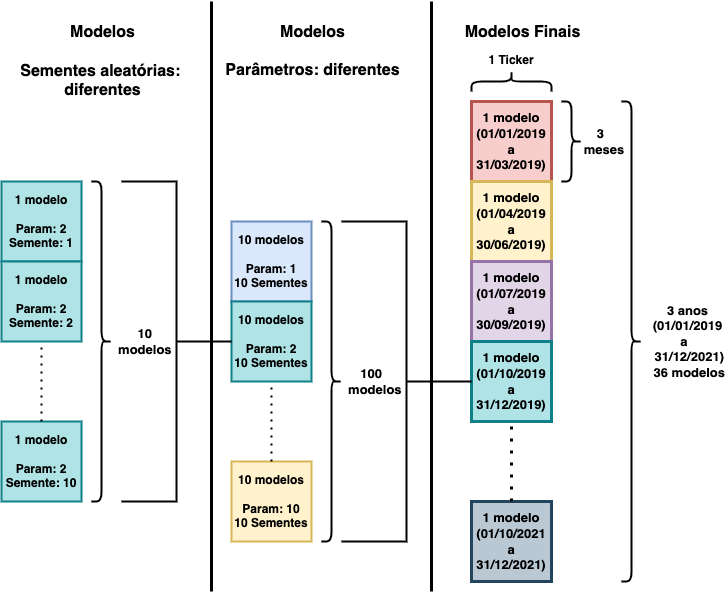
\includegraphics[scale=0.50]{models_chart.png}
    \centering
    \caption{Diagrama de criação de modelos}
    \label{fig:580}
\end{figure}




\FloatBarrier
\subsection{Modelo \textit{Baseline}}
\label{sub:baseline}

\paragraph{} No contexto de ML, entende-se como \textit{baseline} a linha base de comparação de um modelo. Em outras palavras, é uma estratégia simples e de fácil implementação que traz uma performace razoável de se obter na realidade. Neste caso, utilizou-se a média de performance das ações da carteira, ou seja, distribuindo o capital inicial igualmente por cada ação, o rendimento médio destas ações ao longo do tempo é o \textit{baseline}. Não há a consideração de um rebalanceamento dinâmico de capital, isto é, a redistribuição interna do capital das ações que obtiverem maior rendimento para as que obtiverem menor rendimento.

\paragraph{} As Figuras \ref{fig:170} e \ref{fig:927} mostram o \textit{baseline} calculado para os 71 \textit{tickers} indicados na Tabela \ref{tab:5} no intervalo de refinamento dos parâmetros de simulação (01/01/2019 a 31/03/2020) e no intervalo das simulações finais (01/04/2020 a 31/12/2021), respectivamente. Adicionou-se o iBovespa (Seção \ref{sub:ibov}) e o CDI\footnote{Certificado de Depósito Interbancário.} acumulado para fins de comparação. Nota-se a diferença de performance do \textit{baseline} para o iBovespa, o que é razoável já que o \textit{baseline} tem composição fixa e o iBovespa tem uma composição variável tanto na escolha dos ativos quanto em seus respectivos pesos. A Tabela \ref{tab:12} mostra os indicadores de performance para ambos os \textit{baselines}.

\begin{figure}[!htb]
    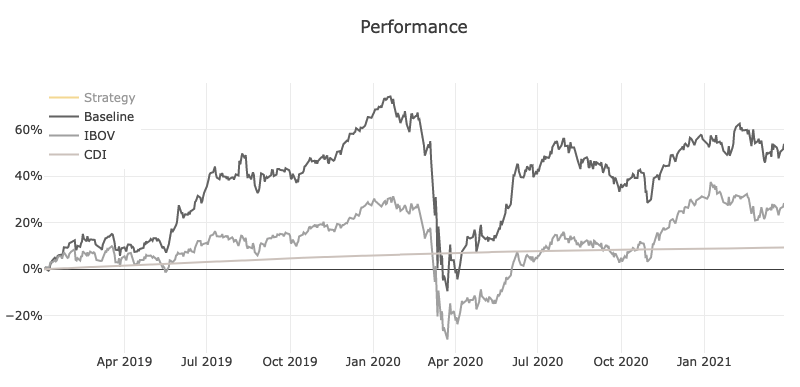
\includegraphics[scale=0.50]{baseline_raw.png}
    \centering
    \caption{Rendimento do \textit{baseline} para o intervalo de 01/01/2019 a 31/03/2020}
    \label{fig:170}
\end{figure}

\begin{figure}[!htb]
    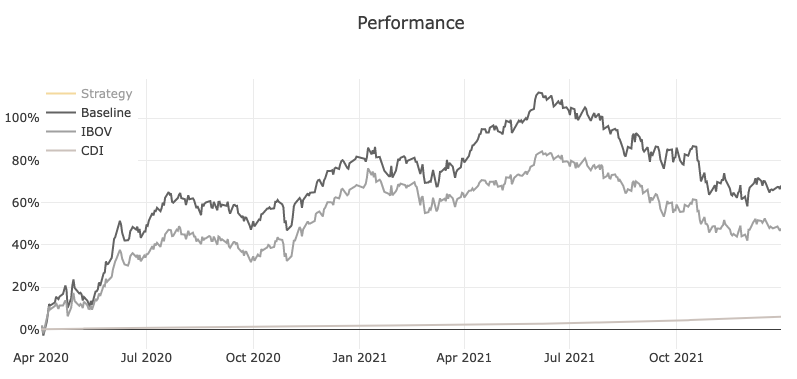
\includegraphics[scale=0.50]{baseline_raw_2.png}
    \centering
    \caption{Rendimento do \textit{baseline} para o intervalo de 01/04/2020 a 31/12/2021}
    \label{fig:927}
\end{figure}

\begin{table}[!htb]
    \begin{center}
        \begin{tabular}{ cc|cccc }
            Início & Fim & Rend. Final & Volatilidade & Sharpe & Sortino \\
            \hline
            01/01/2019 & 31/03/2020 & 6,39\%    & 43,98\% & 0,20 & 0,18 \\
            01/04/2020 & 31/12/2021 & 68,07\%   & 34,84\% & 1,15 & 1,71 \\
        \end{tabular}
        \caption{\textit{Baseline} - Indicadores de Performance}
        \label{tab:12}
    \end{center}
\end{table}




\FloatBarrier
\section{Simulação de Estratégia}
\label{sub:est_simulation}

\FloatBarrier
\subsection{Estrutura}
\label{sub:estrutura}

\paragraph{} O tema escolhido pelo presente trabalho permite uma enorme quantidade possíveis implementações, onde muitas se mostram como promissoras e interessantes de se explorar. No entanto, dar vida a um projeto de engenharia envolve a delimitação de um escopo, que necessariamente restringe as possibilidades. Dessa forma, a Estrutura na qual as estratégias são simuladas se baseia nas seguintes declarações:


\begin{itemize}
    \item Toda estratégia possui um \textbf{capital inicial}, que representa uma quantidade de capital pré-alocado para compra dos ativos financeiros. Essa quantia deve ser sempre respeitada ao longo da simulação de forma a não representar nunca um valor negativo.

    \item Toda estratégia deve possuir uma \textbf{carteira de ativos} (ou lista de ativos) com as respectivas datas iniciais e finais de validade, isto é, intervalos de tempo onde as operações podem ser realizadas. Embora sejam permitidos intervalos diferentes, é convencionado a mesma data de início e de fim para todos os papéis.

    \item Define-se uma  \textbf{operação} como o processo de compra única de um volume de ações de um ativo seguido pela venda de todo o volume comprado, independentemente do tempo, mesmo que esta ocorra em estágios. Nota-se que apenas a venda é cabível de ocorrer em estágios (\textit{i.e.}, venda parcial).

    \item Toda operação possui um \textbf{preço alvo} e um \textbf{\textit{stop loss}}. O preço alvo é um valor acima do preço de compra e o \textit{stop loss} é um valor abaixo do preço de compra. Quando o mercado atinge qualquer um dos dois valores, uma venda é disparada, encerrando a operação em vigor. No entanto, considera-se uma operação de sucesso aquela que encerrou por atingir o preço alvo e uma operação de falha aquela que encerrou por atingir o \textit{stop loss}.

    \item Uma estratégia pode possuir no máximo \textbf{uma operação em vigência} para cada \textit{ticker} em sua bolsa de ativos, portanto para que uma segunda compra ocorra no momento em que já existem papéis adquiridos, é necessários vendê-los primeiro.

    % Relação Risco/Ganho

    \item A \textbf{razão entre ganho e perda}, também denominada relação risco/ganho, é definida por André Moraes \cite{moraes2007se} e predetermina a relação entre o preço alvo e o \textit{stop loss} em qualquer operação. Ela indica a razão entre a diferença do preço alvo \begin{math} P_{target} \end{math} para o preço de compra \begin{math} P_{buy} \end{math} sobre a a diferença do preço de compra para o \textit{stop loss} \begin{math} P_{stop} \end{math} (Equação \ref{eq:50}). O valor recomendado é 3, portanto este é o valor que será utilizado em todo o escopo deste trabalho como uma constante.

    \begin{equation} \label{eq:50}
        G = \dfrac{P_{target} - P_{buy}}{P_{buy} - P_{stop}} = 3
    \end{equation}

    Utiliza-se o termo ``risco de uma operação" ou simplesmente ``risco" como sendo a diferença de valor no qual o \textit{stop loss} é colocado abaixo do preço de compra (Equação \ref{eq:51}). Por exemplo, se o preço de compra de uma operação é de R\$10,00 e o seu risco é de 5\%, então o \textit{stop loss} se encontra em R\$9,50 e o preço alvo em R\$11,50 necessariamente.

    \begin{equation} \label{eq:51}
        Risk = \dfrac{P_{buy} - P_{stop}}{P_{buy}}
    \end{equation}

    \item Não há \textbf{vendas a descoberto}.
    \item Não há \textbf{operações alavancadas}, isto é, um uso temporário de mais capital do que aquele possuído em carteira.

\end{itemize}



\FloatBarrier
\subsection{Premissas}

\paragraph{} As Premissas são um conjunto de afirmações que visam complementar a Estrutura das simulações ao mesmo tempo que garantir a integridade dos resultados, muitas vezes optando pelo pior cenário em situações inconclusivas. São elas:

\begin{itemize}
    \item O momento de decisão de \textbf{entrada em uma operação} por uma estratégia ocorre durante a abertura de mercado do dia corrente, mais precisamente no instante em que o preço de abertura é definido.

    \item No dia que houver a compra de um ativo, não pode haver a venda do mesmo. Em outras palavras, o \textbf{período mínimo de duração de uma operação é de 1 dia útil}.

    \item A \textbf{venda por \textit{timeout}} ocorre quando o número máximo de dias de uma operações extrapola um valor definido (ver Seção \ref{sub:max_op_days})

    \item Devido a ausência de informações mais detalhadas que a janela de tempo diária, a seguinte ordem é priorizada durante a \textbf{venda de um ativo}:

    \begin{enumerate}
        \item Venda por \textit{stop loss}
        \item Venda parcial (caso habilitada)
        \item Venda por preço alvo
        \item Venda por \textit{timeout}
    \end{enumerate}

    \item Caso algum \textbf{preço de venda seja pulado}, ou seja, a descontinuidade entre o preço de abertura do dia corrente e o preço de fechamento do dia anterior não englobe o valor de venda, utiliza-se o preço de abertura do dia corrente. A única exceção acontece para a venda por \textit{timeout}, já que se trata de uma venda compulsória que sempre ocorre no preço de fechamento do dia designado.

\end{itemize}



\FloatBarrier
\subsection{Período Máximo de Dias por Operação}
\label{sub:max_op_days}

\paragraph{} Em teoria, poderia-se permitir que operações não tivessem um período máximo de dias para serem encerradas. Contudo, isso facilmente se prova uma decisão ruim de alocação de capital em ativos que passam por uma fase de consolidação, ou seja, sem qualquer tendência. Além do ativo em questão não encerrar a operação e finalizar seu lucro ou seu prejuízo na carteira, o capital alocado nele não pode ser utilizado por outros ativos que eventualmente venham a lucrar, ou seja, gera-se um efeito de inércia ao aumento da performance geral. Portanto, foi imposto um limite do período de tempo de todas as operação em um valor máximo.

% \paragraph{} A escolha de um número adequado para o limite de dias possui alguns caminhos, resumidos entre os extremos de: um valor fixo geral; ou um valor dinâmico para cada ação. Nota-se que criar um algoritmo que escolha o valor dinâmico a partir da análise dos dados dos últimos meses para cada ação não é trivial. Assim, optou-se por um valor fixo geral, onde a base do estudo se deu na análise ações de perfis opostos.

% \paragraph{} Embora ações de companhias apresentem comportamentos distintos, optou-se por um valor fixo geral, onde o ponto de partida do estudo de um valor adequado se deu através da análise ações de perfis opostos.

\paragraph{} Nesta linha, um algoritmo auxiliar foi criado para varrer um período de dias passados e criar operações com diversos valores de risco, observando quais riscos levariam a operações de sucesso e quais levariam a operações de falha. Também analisou-se a distribuição de operações de sucesso de acordo com os valores de risco e o intervalo de dias corridos.

\paragraph{} De início, foi fixado um intervalo máximo de 90 dias para cada operação hipotética que o algoritmo gerou. O valor é propositalmente excessivo, pois sua função é apenas não forçar \textit{timeout} na maioria das operações. As Figuras \ref{fig:120} e \ref{fig:121} mostram dois histogramas dos dias das operações de sucesso que consideram o menor risco possível, isto é, o menor valor de risco que se pode utilizar a cada dia da série temporal de forma a tornar a operação um sucesso, caso ele exista. Se não existir, é considerado operação de falha, portanto está fora dos histogramas. A legenda indica faixas onde, no caso da linha tracejada em verde na Figura \ref{fig:120}, 50\% das contagens se encontram dentro dos 12 primeiros dias, e assim por diante.

\begin{figure}[!htb]
    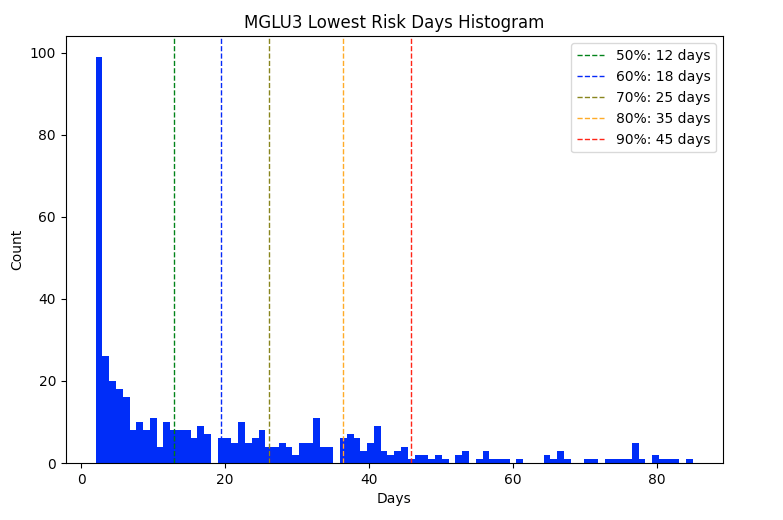
\includegraphics[scale=0.40]{MGLU3_stop_hist_min_risk.png}
    \centering
    \caption{Histograma de dias com risco mínimo em operações de sucesso (01/01/2016 a 31/12/2018) - Companhia: Magazine Luiza (MGLU3)}
    \label{fig:120}
\end{figure}

\begin{figure}[!htb]
    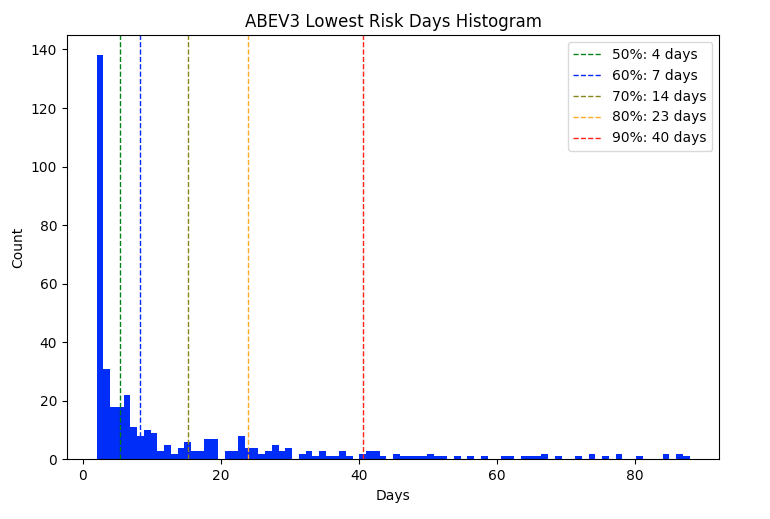
\includegraphics[scale=0.40]{ABEV3_stop_hist_min_risk.png}
    \centering
    \caption{Histograma de dias com risco mínimo em operações de sucesso (01/01/2016 a 31/12/2018) - Companhia: Ambev (ABEV3)}
    \label{fig:121}
\end{figure}

\paragraph{} Também foram analisados os histogramas de risco ótimo por operação, ou seja, o valor de risco que traz o melhor rendimento por operação considerando os dias corridos (Figuras \ref{fig:122} e \ref{fig:123}).

\begin{figure}[!htb]
    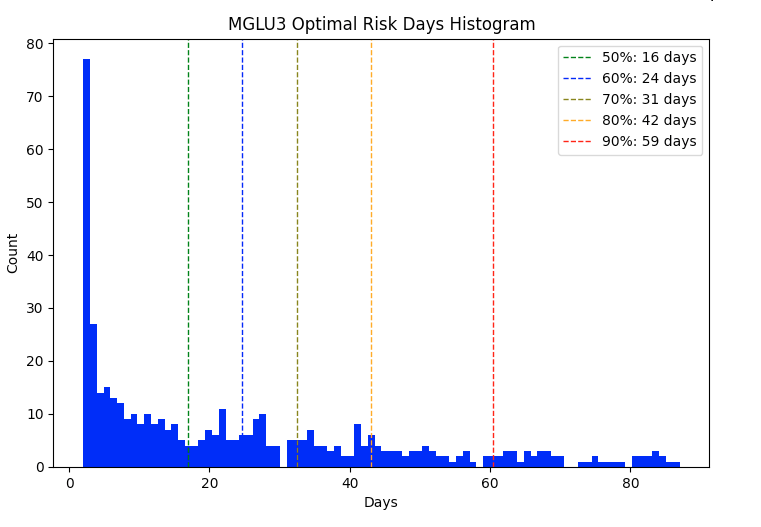
\includegraphics[scale=0.40]{MGLU3_stop_hist_opt_risk.png}
    \centering
    \caption{Histograma de dias com risco ótimo em operações de sucesso (01/01/2016 a 31/12/2018) - Companhia: Magazine Luiza (MGLU3)}
    \label{fig:122}
\end{figure}

\begin{figure}[!htb]
    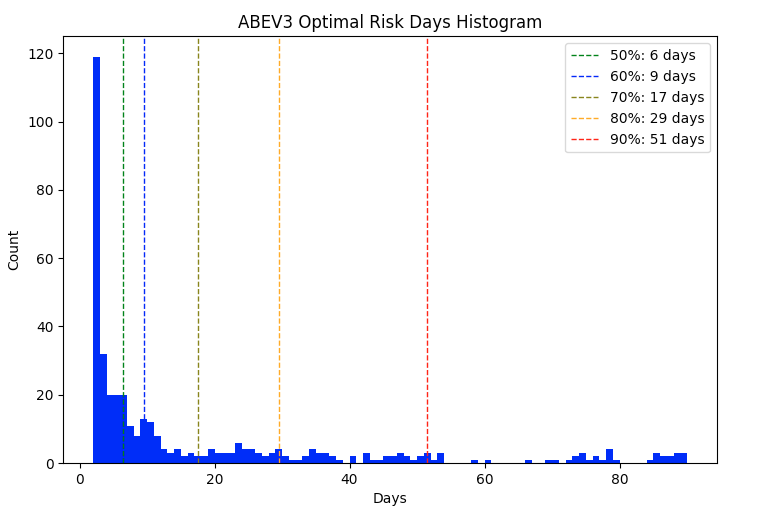
\includegraphics[scale=0.40]{ABEV3_stop_hist_opt_risk.png}
    \centering
    \caption{Histograma de dias com risco ótimo em operações de sucesso (01/01/2016 a 31/12/2018) - Companhia: Ambev (ABEV3)}
    \label{fig:123}
\end{figure}

A Figura \ref{fig:540} mostra a distribuição de todas as operações de sucesso possíveis no intervalo selecionado. Obseva-se que valores baixos de risco não costumam estar associados a longos períodos de operação e que a maior densidade de operações de sucesso se encontra em baixo risco e em baixa duração de operação.

\begin{figure}[!htb]
    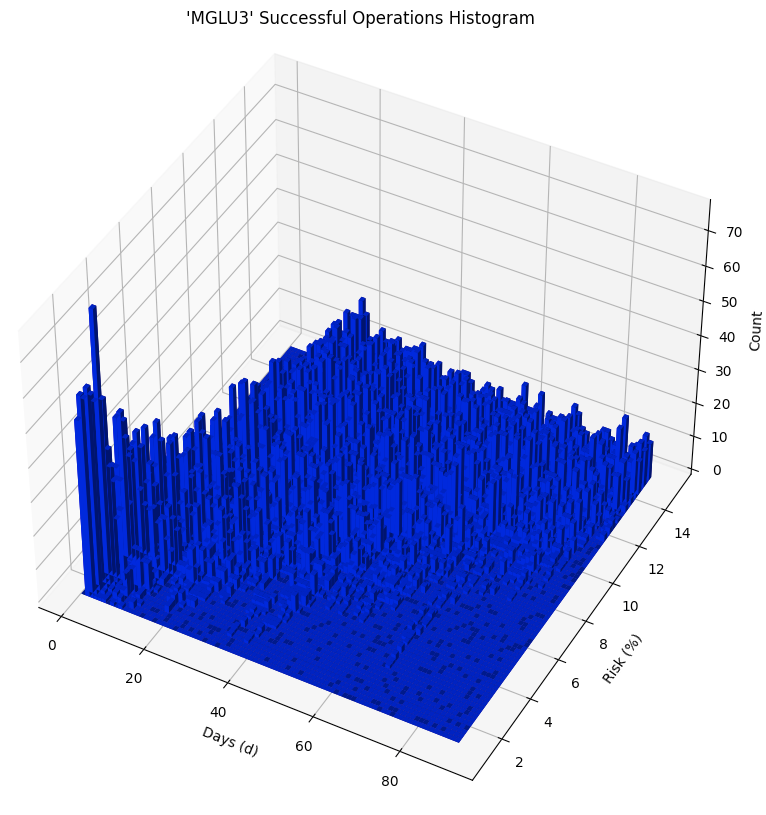
\includegraphics[scale=0.40]{riskmap_mglu3.png}
    \centering
    \caption{MGLU3 - Histograma de todas as operações de sucesso (01/01/2016 a 31/12/2018)}
    \label{fig:540}
\end{figure}

A Tabela \ref{tab:4} resume o período de dias que engloba 90\% das contagens dos histogramas conforme indicado nas Figuras \ref{fig:120}, \ref{fig:121}, \ref{fig:122} e \ref{fig:123}.

\begin{table}[h!]
    \begin{center}
        \begin{tabular}{ c|cc }
            & Menor Risco & Risco Ótimo \\
            \hline
            MGLU3 & 45 dias & 59 dias \\
            ABEV3 & 40 dias & 51 dias \\
        \end{tabular}
        \caption{Período de dias que engloba 90\% das contagens dos histogramas}
        \label{tab:4}
    \end{center}
\end{table}

\paragraph{} Com base nos valores encontrados, foi escolhido o período máximo de \textbf{45 dias} para qualquer operação.

% \paragraph{} Na tentativa de encontrar o valor bem ajustado para o Período Máximo de Dias, uma simulação com o parâmetro ajustado para o intervalo de 1 a 90 dias foi executada para os 71 \textit{tickers} da Tabela \ref{tab:5} para o período de 01/01/2019 a 31/12/2021. Utilizou-se um RCC de 0,22\% para evitar saturação de capital e nenhuma otimização. A Figura \ref{fig:740} mostra os resultados obtidos. Os máximos dos indicadores de performance coincidem em 45 dias de Período Máximo de Dias uma vez que os modelos utilizados na simulação foram criados a partir de \textit{datasets} que utilizavam este valor como limite de suas operações artificiais (Seção \ref{sub:dataset_gen}).

% % ID: [101, 190]
% \begin{figure}[!htb]
%     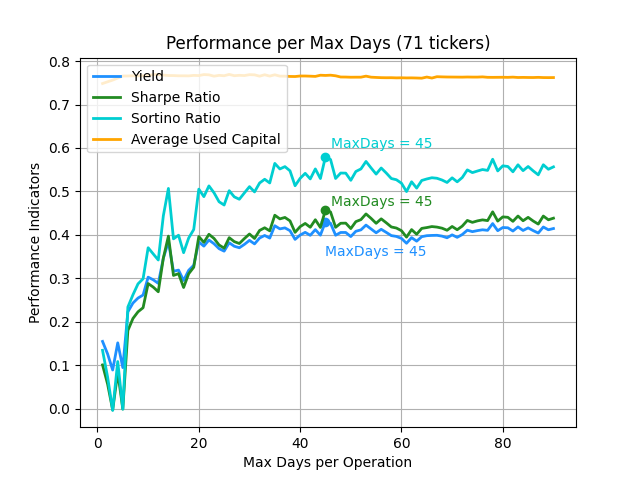
\includegraphics[scale=0.80]{performance_per_max_days.png}
%     \centering
%     \caption{Análise do Período Máximo de Dias por Operação (71 \textit{tickers} - 01/01/2019 a 31/12/2021)}
%     \label{fig:740}
% \end{figure}



\FloatBarrier
\subsection{Margem de Risco}
\label{sub:operation_risk}

\paragraph{} A Margem de Risco é encontrada a partir de um valor intermediário entre o Risco Mínimo e o Risco Máximo.

\paragraph{} Pelo fato da metodologia de cálculo do Risco Máximo e do Risco Mínimo seguirem raciocínios diferentes (Seção \ref{sub:features}), podem ocorrer momentos nos quais a equação \begin{math} Risk_{max} < Risk_{min} \end{math} seja verdadeira, em outras palavras, as ondas de subida de preço entre picos no gráfico diário não compensem as oscilações inerentes ao ruído diário dos \textit{candlesticks}. Enquanto este evento ocorrer, não haverá entrada em operações para o ativo envolvido.

\paragraph{} Para a maioria dos casos, tem-se \begin{math} Risk_{max} > Risk_{min} \end{math}. O valor da Margem de Risco (\begin{math} Risk_{operation} \end{math}) é definido pelo parâmetro \begin{math} Risk_{coef} \end{math} de acordo com a Equação \ref{eq:70}, onde \begin{math} 0 \le Risk_{coef} \le 1 \end{math}.

\begin{equation} \label{eq:70}
    Risk_{operation} = Risk_{min} + Risk_{coef}(Risk_{max} - Risk_{min})
\end{equation}

\paragraph{} A Figura \ref{fig:553} resume as simulações cujos valores de Margem de Risco estão no intervalo fechado [0.10, 0.70]. Foram utilizados os 71 \textit{tickers} da Tabela \ref{tab:5} no período de 01/01/2019 a 31/03/2020, além do Período Máximo de Dias por Operação de 45 dias (refinado na Seção \ref{sub:max_op_days}). Utilizou-se um RCC de 0,10\% apenas para evitar saturação de capital. Nota-se que o ponto de máximo para o índice de Sharpe e o índice de Sortino coincidiu para a Margem de Risco de 0,43, que será o valor escolhido para as simulações seguintes. Apesar do ponto de máximo do rendimento final indicar o parâmetro de 0,25, este valor não será considerado pois o índice de Sharpe é uma alternativa mais robusta que engloba o anterior e considera também outros efeitos.

% ID: [1, 100]
\begin{figure}[!htb]
    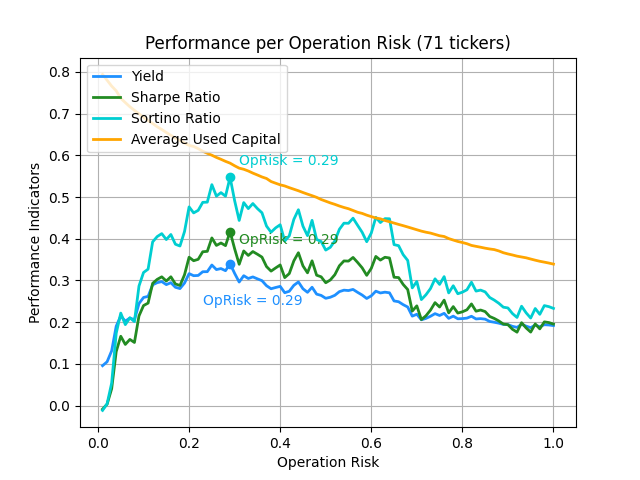
\includegraphics[scale=0.80]{performance_per_op_risks.png}
    \centering
    \caption{Indicadores de performance em função da Margem de Risco (71 tickers, 01/01/2019 a 31/03/2020)}
    \label{fig:553}
\end{figure}



\FloatBarrier
\subsection{Gerenciamento de Risco}
\label{sub:risk_man}

\paragraph{} Segundo André Moraes \cite{moraes2007se}, um bom Gerenciamento de Risco é essencial para a performance de uma estratégia. Afinal, não adianta obter uma alta taxa de acerto em operações de cujo lucro médio não compense as perdas acumuladas pelas operações que falham. Além disso, estar com o capital muito alocado em ativos de um único segmento é perigoso devido à exposição à fatores como falta de insumos industriais, mudanças na legislação, crises internas, instabilidade política, dentre outros.

\paragraph{} Para mitigar as questões levantadas, algumas medidas foram tomas inspiradas no trabalho de André Moraes \cite{moraes2007se}. São elas:

\begin{itemize}
    \item Diversificação de ativos em segmentos de mercado variados através da escolha de um alto número de \textit{tickers} na carteira, mais especificamente 71.
    \item Criação do Coeficiente de Risco-Capital\footnote{ou \textit{Risk-Capital Coefficient} (RCC)}
\end{itemize}

\paragraph{} O Coeficiente de Risco-Capital, definido pela Equação \ref{eq:60}, é uma constante que equilibra a relação entre o capital de entrada em uma operação e o risco escolhido. Seu valor é configurado previamente no Arquivo de Configuração (ver Tabela \ref{tab:3}) e vale para todos os ativos da carteira.

\begin{equation} \label{eq:60}
    RCC = Capital \times Risk
\end{equation}

\paragraph{} Durante uma simulação, a estratégia primeiro encontra o valor do risco desejado para entrar na operação, depois escolhe o capital a ser alocado. Dessa forma, a Equação \ref{eq:61} mostra de fato a aplicação do RCC. É evidente que quanto maior o risco envolvido, menor o capital a ser alocado e vice-versa.

\begin{equation} \label{eq:61}
    Capital = \dfrac{RCC}{Risk}
\end{equation}

\paragraph{} O RCC influencia diretamente no uso médio de capital de uma estratégia. Por um lado, um uso de capital baixo significa um mau aproveitamento do capital, o que leva a uma performance ruim. Por outro lado, muito uso de capital implica em pouco capital disponível para entrada em novas operações, o que também leva a uma performance ruim e instável, visto que a operação que iniciar imediatamente antes das demais leva quase todos o capital consigo.

\paragraph{} A Figura \ref{fig:550} mostra o gráfico da relação entre os indicadores de performance em função do RCC para diversas simulações. Foi considerado o período de 01/01/2019 a 31/03/2020, os 71 \textit{tickers} da Tabela \ref{tab:5}, a Margem de Risco de 0,43 (refinado na Seção \ref{sub:operation_risk}) e o Período Máximo de Dias por Operação de 45 dias (refinado na Seção \ref{sub:max_op_days}). Notam-se duas regiões de máximos locais no início e no fim do gráfico, onde os valores de RCC são 0,11\% e 6,10\%, respectivamente. Percebe-se também que a partir do RCC de 1,00\%, o uso médio de capital por estratégia começa a saturar e o número percentual de operações totais começa a cair significativamente. Este efeito ocorre devido à falta de capital disponível para novas operações em momentos de saturação. Ou seja, quanto mais a direita no gráfico, menos operações são efetuadas e maior é o desvio padrão do capital de aporte nas operações restantes.

% ID: [62, 181]
\begin{figure}[!htb]
    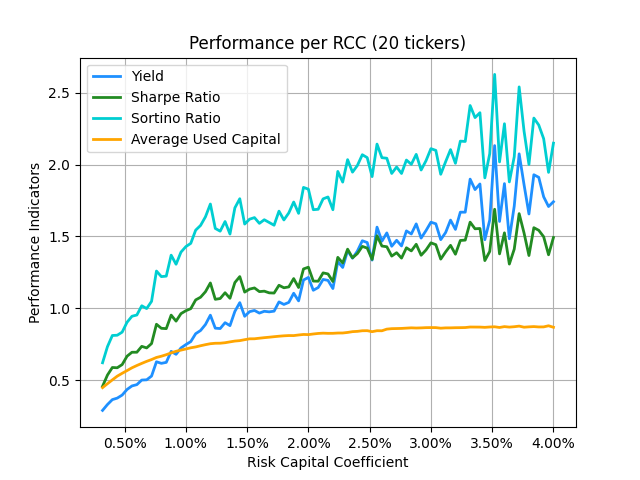
\includegraphics[scale=0.80]{performance_per_rcc.png}
    \centering
    \caption{Indicadores de performance em função do RCC (71 tickers: 01/01/2019 a 31/03/2020)}
    \label{fig:550}
\end{figure}

\paragraph{} A Tabela \ref{tab:465} mostra uma análise estatística do capital de entrada em operações para ambas as regiões de máximo local. Conforme esperado, o devio padrão cresce bastante, o que mostra que as operações estão com um aporte de capital elevadíssimo e assim que são finalizadas, o primeiro modelo da fila a indicar compra recebe quase todo o capital disponível. Por outro lado, tanto as operações que antes seriam finalizadas com sucesso quanto as que seriam finalizadas com falha são igualmente prejudicadas.

\begin{table}[h!]
    \begin{center}
        \begin{tabular}{ c|c|cc }
            RCC & Uso Médio         & Média de Capital          & Desvio Padrão do Capital \\
                & de Capital Geral  & de Entrada por Operação   & de Entrada por Operação \\
                % &  & por Operação & por Operação \\
            \hline
            0,11\% & 56,85\% & R\$1188,89 & R\$449,74 \\
            6,10\% & 99,64\% & R\$4304,55 & R\$26584,57 \\
        \end{tabular}
        \caption{Análise estatística do capital de entrada em operações para as regiões de máximo local}
        \label{tab:465}
    \end{center}
\end{table}

\paragraph{} Pode-se caracterizar o primeiro pico (RCC de 0,11\%) como uma região de predominância mais uniforme dos modelos gerados, pois toda ordem de compra é acatada com capitais de entrada razoavelmente próximos entre si. O custo disso são os baixos valores dos indicadores de performance. Já o segundo pico (RCC de 6,10\%) está situado na região de melhor performance, porém é onde a clareza operacional dos modelos pode ser questionada, pois não é fácil distinguir o quanto o efeito aparentemente aleatório da alavancagem de algumas operações em detrimento de outras entrou em simbiose com a operação dos modelos gerados.

\paragraph{} Dentre as execuções que compõem a Figura \ref{fig:550}, extraiu-se os gráficos de rendimento e de uso de capital para as simulações de RCC=0.11\% e RCC=6,01\% (Figuras \ref{fig:551}, \ref{fig:552}, \ref{fig:789} e \ref{fig:790}, respectivamente). Assim, é possível verificar visualmente as questões levantadas.

\begin{figure}[!htb] % ID: 73
    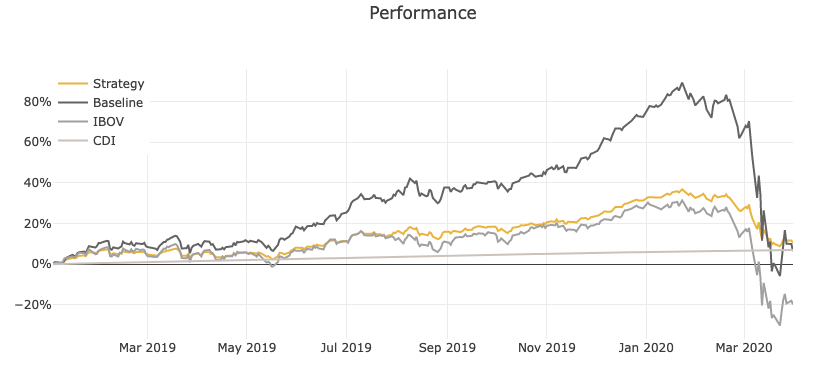
\includegraphics[scale=0.50]{performance_rcc_0_11p.png}
    \centering
    \caption{Rendimento (71 tickers, 01/01/2019 a 31/03/2020, RCC = 0,11\%)}
    \label{fig:551}
\end{figure}

\begin{figure}[!htb] % ID: 172
    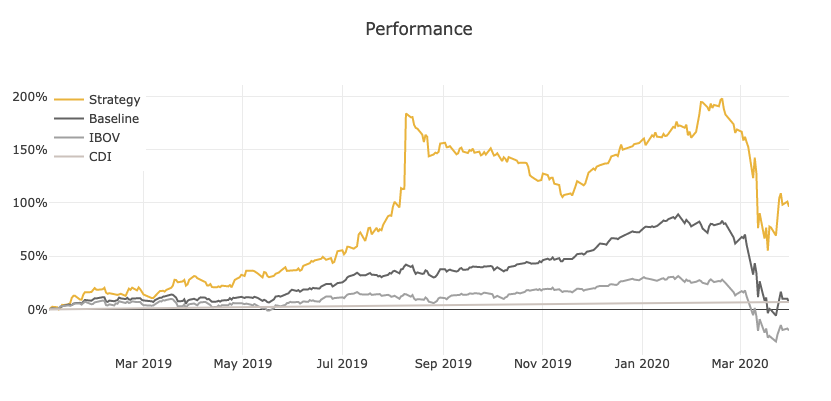
\includegraphics[scale=0.50]{performance_rcc_6_1p.png}
    \centering
    \caption{Rendimento (71 tickers, 01/01/2019 a 31/03/2020, RCC = 6,10\%)}
    \label{fig:552}
\end{figure}

\begin{figure}[!htb] % ID: 73
    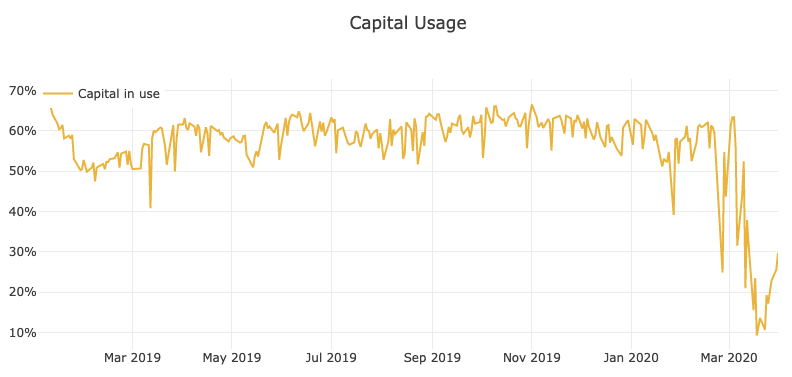
\includegraphics[scale=0.50]{rcc_capital_usage_0_11p.png}
    \centering
    \caption{Uso de Capital (71 tickers, 01/01/2019 a 31/03/2020, RCC = 0,11\%)}
    \label{fig:789}
\end{figure}

\begin{figure}[!htb] % ID: 172
    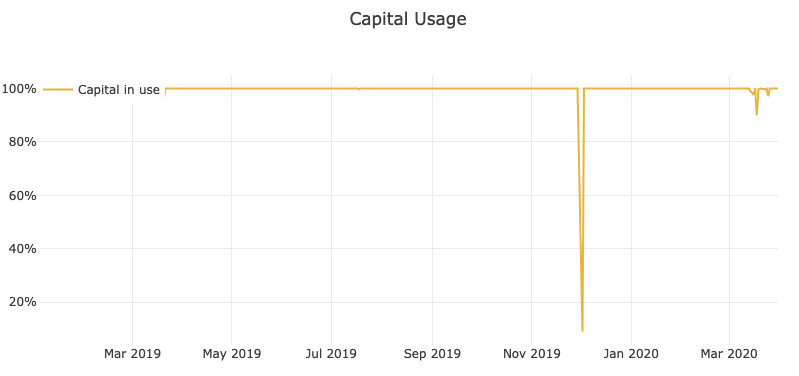
\includegraphics[scale=0.50]{rcc_capital_usage_6_10p.png}
    \centering
    \caption{Uso de Capital (71 tickers, 01/01/2019 a 31/03/2020, RCC = 6,10\%)}
    \label{fig:790}
\end{figure}

\paragraph{} Um problema geral e inerente à abordagem do RCC é a necessidade do conhecimento \textit{a priori} de um valor razoável. Ou seja, sem algumas simulações prévias, não há como se ter indícios de um valor refinado. Uma proposta para se atenuar esse problema é através da criação de um controle proporcional que aumente o RCC geral em função do baixo aproveitamento do uso de capital ao longo dos dias e vice-versa. Essa alternativa também é chamada de RCC Dinâmico e abordada em mais detalhes na Seção \ref{sub:dynamic_rcc}.



\FloatBarrier
\subsection{Controle Proporcional para Uso de Capital}
\label{sub:dynamic_rcc}

\paragraph{} A criação de um RCC fixo pode ser interessante do ponto de vista de Gerenciamento de Risco, mas na prática deixa um pouco a desejar por requerer uma noção prévia de um valor adequado. Esse valor só pode vislumbrado através de simulações anteriores ao período desejado, onde o comportamento do mercado pode ser significativamente diferente a ponto de requerer um novo RCC, dificultando um bom ajuste. Em outras palavras, apenas um RCC fixo pode levar a problemas de subaproveitamento do Uso de Capital da carteira.

\paragraph{} Uma forma de se atenuar esse problema é através da criação de um RCC Dinâmico, configurado através de um Controle Proporcional. A vantagem dessa abordagem está na diminuição da sensibilidade do RCC em relação à performance geral, permitindo um ajuste menos preciso sem grande impacto de performance. O Controle atua no rebalanceamento de capital em função do uso médio de capital vigente, ou seja, períodos com mais disponibilidate de capital terão uma maior alavancagem.

\paragraph{} As Equações \ref{eq:100} e \ref{eq:101} mostram o cálculo do erro e do RCC dinâmico (\begin{math} RCC_{din} \end{math}) a partir do valor de referência para o uso médio de capital (\begin{math} C_{ref} \end{math}), do uso médio de capital dos últimos 10 dias de simulação (\begin{math} \overline{C_{10d}} \end{math}), do RCC fixo (\begin{math} RCC \end{math}, definido pela Equação \ref{eq:60}) e da constante de ganho proporcional (\begin{math} K \end{math}).

\begin{equation} \label{eq:100}
    e = C_{ref} - \overline{C_{10d}}, \quad \mbox{para } 0 \le C_{ref}\le 1, \mbox{e } 0 \le \overline{C_{10d}} \le 1
\end{equation}

\begin{equation} \label{eq:101}
    RCC_{din} = RCC (1 + K e)
\end{equation}

% \paragraph{} Foi utilizado \begin{math} C_{ref} = 1.0 \end{math}, \begin{math} K = 10 \end{math} e \begin{math} RCC_{fix} = 0.003 \end{math}

% \paragraph{} A Figura \ref{fig:150} mostra o ganho de performance obtido pela implementação do RCC Dinâmico com os valores \begin{math} C_{ref} = 1.0 \end{math}, \begin{math} K = 7,5 \end{math} e \begin{math} RCC_{fix} = 0.0022 \end{math}. A linha em amarelo indica a simulação com uso do RCC Dinâmico enquanto a linha verde indica a simulação sem o uso. Nenhuma outra otimização foi utilizada. A Tabela \ref{tab:10} traz um comparativo dos resultados das simulações. Nota-se que o RCC foi ajustado para que o Uso Médio de Capital de ambas simulações ficassem próximos.

% % ID: 420 (sem), 419 (com)
% \begin{figure}[!htb]
%     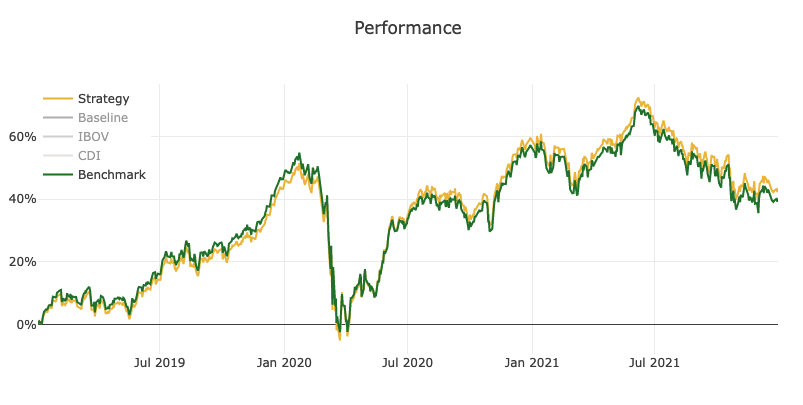
\includegraphics[scale=0.50]{dyn_rcc_no_flags.png}
%     \centering
%     \caption{Performance por uso de RCC dinâmico sem \textit{flags} de descanso}
%     \label{fig:150}
% \end{figure}

% \begin{table}[h!]
%     \begin{center}
%         \begin{tabular}{ c|cc|ccc }
%             RCC Din. & RCC fixo & Uso Méd. Cap. & Rend. Final & Sharpe & Sortino \\
%             \hline
%             Não & 0,50\% & 84,20\% & 44,93\% & 0,44 & 0,53 \\
%             Sim & 0,22\% & 84,11\% & 47,37\% & 0,47 & 0,57 \\
%         \end{tabular}
%         \caption{RCC Dinâmico - Comparação de Resultados sem \textit{flags} de descanso}
%         \label{tab:10}
%     \end{center}
% \end{table}

% \paragraph{} Analogamente à Figura \ref{fig:150}, a Figura \ref{fig:151} também mostra o ganho de performance, porém na condição de ativação dos Descansos por Tendência de Baixa e por Identificação de Crises para ambas as simulações. A Tabela \ref{tab:11} compara os resultados das simulações.

% % ID: 425 (sem), 422 (com)
% \begin{figure}[!htb]
%     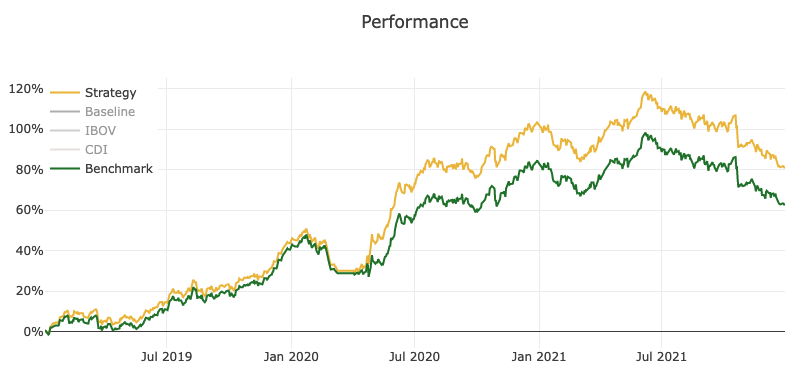
\includegraphics[scale=0.50]{dyn_rcc_with_flags.png}
%     \centering
%     \caption{Performance por uso de RCC dinâmico com \textit{flags} de descanso}
%     \label{fig:151}
% \end{figure}

% \begin{table}[h!]
%     \begin{center}
%         \begin{tabular}{ c|cc|ccc }
%             RCC Din. & RCC fixo & Uso Méd. Cap. & Rend. Final & Sharpe & Sortino \\
%             \hline
%             Não & 0,63\% & 73,89\% & 66,61\% & 0,94 & 1,27 \\
%             Sim & 0,22\% & 73,98\% & 83,38\% & 1,20 & 1,69 \\
%         \end{tabular}
%         \caption{RCC Dinâmico - Comparação de Resultados com \textit{flags} de descanso}
%         \label{tab:11}
%     \end{center}
% \end{table}

\paragraph{} A fim de simplificar a análise, o valor de \begin{math} C_{ref} \end{math} foi configurado como 100\%, deixando o processo de refinamento para os parâmetros RCC e K. Como ambos influenciam diretamente o uso de capital e todos os indicadores de performance, foram acoplados e analisados conjuntamente através das curvas de \begin{math} RCC \times K \end{math}.

\paragraph{} As Figuras \ref{fig:152}, \ref{fig:153} e \ref{fig:154} apresentam indicadores de performance para valores de RCC e de K diferentes. Nessas simulações foram utilizados os 71 \textit{tickers} indicados na Tabela \ref{tab:5} no intervalo de 01/01/2019 a 31/03/2020, junto com a Margem de Risco de 0,43 (refinado na Seção \ref{sub:operation_risk}) e o Período Máximo de Dias por Operação de 45 dias (refinado na Seção \ref{sub:max_op_days}).

\paragraph{} A primeira e mais notório observação que se pode fazer pelas Figuras \ref{fig:152} e \ref{fig:153} é que a região de melhor performance se encontra com baixo RCC e alto K. Também é possível verificar que o aumento graduau das curvas \begin{math} RCC \times K \end{math} encontrou um comportamento assintótico a partir de 1,40.

\paragraph{} De forma semelhante ao comportamento observado na Seção \ref{sub:risk_man}, a Figura \ref{fig:154} mostra a tendência de saturação do uso médio de capital com o aumento do RCC e a suavização desse efeito que ocorre ao se diminuir a importância do RCC e aumentar a do K. Já a Figura \ref{fig:155} deixa claro que tanto aumentando o RCC quanto o K, em algum momento o número de operações totais cairá, porém é visível a presença de um ponto de máximo na região de \begin{math} K=500 \end{math} e \begin{math} RCC=[0,08\%; 0,40\%] \end{math} em cada curva.

% Falar do comportamento assintotico e escolha do RCCxK = 1,8

\paragraph{} Um segundo reflexo do efeito mencionado de suavização da saturação de capital através do aumento do K se faz presente na dimnuição do desvio padrão do capital de entrada por operação. Assim como foi tratado na Seção \ref{sub:risk_man} pela Tabela \ref{tab:465}, a Tabela \ref{tab:466} mostra os valores de média e desvio padrão do capital de entrada por operação, porém neste caso para as simulações de \begin{math} RCC \times K = 1,80 \end{math}.

\begin{table}[h!]
    \begin{center}
        \resizebox{\textwidth}{!}{
        \begin{tabular}{ c|c|c|cc }
            RCC & K & Uso Médio         & Média de Capital          & Desvio Padrão do Capital \\
                & K & de Capital Geral  & de Entrada por Operação   & de Entrada por Operação \\
            \hline
            0,11\% & - & 56,85\% & R\$1188,89 & R\$449,74 \\
            6,10\% & - & 99,64\% & R\$4304,55 & R\$26584,57 \\
            \hline
            0,000576\% & 312500 & 0.9721 & R\$2411,92 & R\$12306,90 \\
            0,002880\% & 62500 & 0.9725 & R\$2485,83 & R\$12107,00 \\
            0,014400\% & 12500 & 0.9767 & R\$2509,47 & R\$10650,77 \\
            0,072000\% & 2500 & 0.9798 & R\$2396,77 & R\$9554,60 \\
            0,360000\% & 500 & 0.9846 & R\$2332,00 & R\$7446,53 \\
            1,800000\% & 100 & 0.9896 & R\$2533,79 & R\$8617,72 \\
        \end{tabular}}
        \caption{Análise estatística do capital de entrada em operações para \begin{math} RCC \times K = 1,80 \end{math}}
        \label{tab:466}
    \end{center}
\end{table}

% Estratégia escolhida: ID 226

% ID: [182, 235]
\begin{figure}[!htb]
    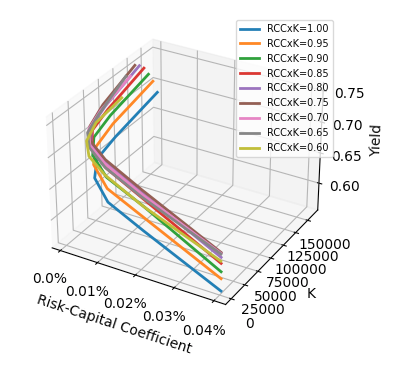
\includegraphics[scale=0.70]{yield_per_rcc_k.png}
    \centering
    \caption{Rendimento final sob uso de RCC dinâmico}
    \label{fig:152}
\end{figure}

% ID: [182, 235]
\begin{figure}[!htb]
    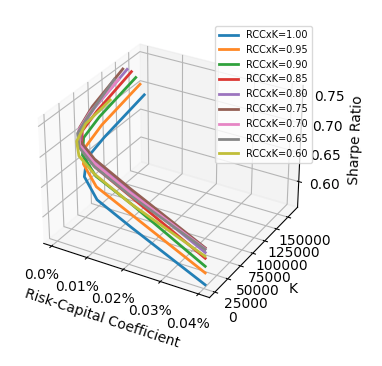
\includegraphics[scale=0.70]{sharpe_per_rcc_k.png}
    \centering
    \caption{Índice de Sharpe sob uso de RCC dinâmico}
    \label{fig:153}
\end{figure}

% ID: [182, 235]
\begin{figure}[!htb]
    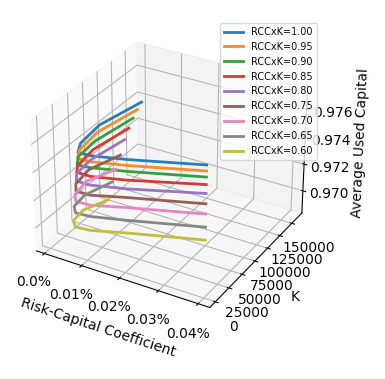
\includegraphics[scale=0.70]{avgcap_per_rcc_k.png}
    \centering
    \caption{Uso médio de capital sob uso de RCC dinâmico}
    \label{fig:154}
\end{figure}

% ID: [182, 235]
\begin{figure}[!htb]
    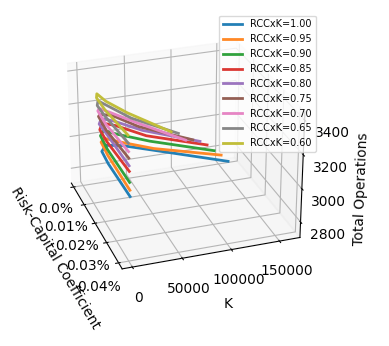
\includegraphics[scale=0.70]{totalop_per_rcc_k.png}
    \centering
    \caption{Total de operações sob uso de RCC dinâmico}
    \label{fig:155}
\end{figure}

\paragraph{} Por fim, chama-se atenção para dois pares de valores de \begin{math} RCC \times K \end{math}. O primeiro par é mostrado pela curva \begin{math} RCC \times K = 1,80 \end{math} no ponto maior índice de Sharpe (\begin{math} RCC = 0,00288\%, K = 62500 \end{math}). Este curva foi escolhida, pois a partir de \begin{math} RCC \times K = 1,40 \end{math}, tanto o índice de Sharpe quanto o rendimento começam a apresentar um comportamento assintótico, não sendo necessário escolher uma curva de valor muito mais alto que este. Já o segundo par foi escolhido a partir do máximo local encontrado na curva \begin{math} RCC \times K = 0,10 \end{math} da Figura \ref{fig:155} (\begin{math} RCC = 0,1\%, K = 100 \end{math}). Este, por sua vez, foi escolhido para representar a região de menor quantidade de operações perdidas.



\FloatBarrier
\subsection{Lista de Parâmetros de Configuração}
\label{sub:params_list}

\paragraph{} A Tabela \ref{tab:3} mostra uma lista de todos os parâmetros configuráveis em uma simulação. Nota-se que as variáveis de escopo geral são aplicáveis a toda e qualquer estratégia presente no Arquivo de Configuração enquanto as variáveis de escopo local dizem respeito apenas a um grupo de estratégias em parciluar (ver Seção \ref{sub:conf_file}).

{\small
\begin{longtable}[m]{| m{11em} | m{21em} |}
    \caption{Lista de parâmetros de simulação\label{tab:3}}\\

    \hline
    Nome do Parâmetro & Descrição \\
    \hline
    \endfirsthead

    \hline
    \multicolumn{2}{|c|}{Continuação da Tabela \ref{tab:3}} \\
    \hline
    Nome do Parâmetro & Descrição \\
    \hline
    \endhead

    \hline
    \endfoot

    \hline
    \multicolumn{2}{|c|}{Fim da Tabela \ref{tab:3}} \\
    \hline
    \endlastfoot

    \hline
    % show\_results & Geral & Exibe \textit{dashboard} da última simulação completada ao final. Tipo: \textit{Boolean}. \textit{Default}: \textit{True}. Listável: Não. \\
    % \hline
    % min\_risk\_features & Geral & Risco mínimo para o cálculo de \textit{features}. Tipo: \textit{Float}. \textit{Default}: 0,01. Listável: Não. \\
    % \hline
    % max\_risk\_features & Geral & Risco máximo para o cálculo de \textit{features}. Tipo: \textit{Float}. \textit{Default}: 0,10. Listável: Não. \\
    % \hline
    \textbf{name} & \textbf{(OBRIGATÓRIO)} Nome da estratégia a ser executada. Único valor válido: ``ML". Tipo: \textit{String}. Listável: Não. \\
    \hline
    \textbf{alias} & \textbf{(OBRIGATÓRIO)} Rótulo de Identificação. Tipo: \textit{String}. \textit{Default}: \textit{String} vazia. Listável: Não. \\
    \hline
    \textbf{stock\_targets} & \textbf{(OBRIGATÓRIO)} \textit{Array} de ações a incluir na carteira. Formato indicado pela Figura \ref{fig:101}. \\
    \hline
    comment & Comentário. Tipo: \textit{String}. \textit{Default}: \textit{String} vazia. Listável: Não. \\
    \hline
    capital & Capital total da carteira em reais (R\$). Tipo: \textit{Float}. \textit{Default}: 100000. Listável: Sim. \\
    \hline
    risk\_capital\_coefficient & Coeficiente de risco-capital (RCC) geral (Seção \ref{sub:risk_man}). Tipo: \textit{Float}. \textit{Default}: 0,001. Listável: Sim. \\
    \hline
    % tickers\_bag & Critério de escolha do grupo de ativos a escolher dentro de ``stock\_targets". Valores aceitos: ``listed\_first" (ordem de listagem); ``random" (ordem aleatória). \textit{Default}: ``listed\_first". Listável: Sim. \\
    % \hline
    % tickers\_number & Número de ativos a escolher dentro de ``stock\_targets", de acordo com ``tickers\_bag". Tipo: \textit{Int}. \textit{Default}: 0 (todos). Listável: Sim. \\
    % \hline
    tickers\_number & Número de ativos a escolher dentro de ``stock\_targets" em ordem de listagem. Tipo: \textit{Int}. \textit{Default}: 0 (todos). Listável: Sim. \\
    \hline
    min\_order\_volume & Volume mínimo por operação. Tipo: \textit{Int}. \textit{Default}: 1. Listável: Sim. \\
    \hline
    % gain\_loss\_ratio & Razão entre ganho e perda. Para uma unidade de risco (delta pencentual entre preço de compra e \textit{stop loss}) são utilizadas N unidades de risco acima no preço preço de compra para definir o preço alvo. Tipo: \textit{Float}. \textit{Default}: 3. Listável: Sim. \\
    % \hline
    max\_days\_per\_operation & Número máximo de dias por operação (Seção \ref{sub:max_op_days}). Inclui o dia de compra. Caso excedido, ocorre venda compulsória pelo preço de fechamento no último dia da contagem. Tipo: \textit{Int}. \textit{Default}: 45. Listável: Não. \\
    \hline
    min\_risk & Risco mínimo por operação. Tipo: \textit{Float}. \textit{Default}: 0,003. Listável: Sim. \\
    \hline
    max\_risk & Risco máximo por operação. Tipo: \textit{Float}. \textit{Default}: 0,15. Listável: Sim. \\
    \hline
    operation\_risk & Margem de Risco (Seção \ref{sub:operation_risk}). Tipo: \textit{Float}. \textit{Default}: 0,5. Listável: Sim. \\
    \hline
    % enable\_frequency\hspace{2em} \_normalization & Uso de normalização por frequência de operações (Seção \ref{sub:freq_norm}). Tipo: \textit{Boolean}. \textit{Default}: \textit{False}. Listável: Sim. \\
    % \hline
    % enable\_profit\hspace{4em} \_compensation & Uso de compensação por lucratividade acumulada (Seção \ref{profit_comp}). Tipo: \textit{Boolean}. \textit{Default}: \textit{False}. Listável: Sim. \\
    % \hline
    % enable\_downtrend\_halt & Uso de descanso por identificação de tendência de baixa (Seção \ref{sub:downtrend_halt}). Tipo: \textit{Boolean}. \textit{Default}: \textit{False}. Listável: Sim. \\
    % \hline
    % enable\_crisis\_halt & Uso de descanso por identificação de crises (Seção \ref{sub:crisis_halt}). Tipo: \textit{Boolean}. \textit{Default}: \textit{False}. Listável: Sim. \\
    % \hline
    enable\_dynamic\_rcc & Uso de Coeficiente de Risco-Capital dinâmico (Seção \ref{sub:dynamic_rcc}). Tipo: \textit{Boolean}. \textit{Default}: \textit{False}. Listável: Sim. \\
    \hline
    dynamic\_rcc\_reference & Valor de referência de uso de capital médio no controle do RCC dinâmico (Seção \ref{sub:dynamic_rcc}). Tipo: \textit{Float}. \textit{Default}: 1,0. Listável: Sim. \\
    \hline
    dynamic\_rcc\_k & Valor do ganho proporcional K no controle do RCC dinâmico (Seção \ref{sub:dynamic_rcc}). Tipo: \textit{Float}. \textit{Default}: 10. Listável: Sim. \\
    \hline

    % purchase\_margin & Margem percentual aplicada ao valor de compra. Ex: Se o alvo de compra estiver configurado para R\$100, uma margem de 1\% permitirá a compra antecipada em R\$99. Tipo: \textit{Float}. \textit{Default}: 0. Listável: Sim. \\
    % \hline
    % stop\_margin & Margem percentual aplicada ao valor do \textit{stop loss}. Ex: Se o \textit{stop} estiver configurado para R\$100, uma margem de 1\% permitirá a compra antecipada em R\$101. Tipo: \textit{Float}. \textit{Default}: 0. Listável: Sim. \\
    % \hline
    % partial\_sale & Uso de saídas parciais. Tipo: \textit{Boolean}. \textit{Default}: \textit{False}. Listável: Sim. \\
    % \hline
    % stop\_type & Tipo de \textit{stop loss} utilizado. Valores aceitos: ``normal"; ``staircase" (para cada patamar de unidade de risco que o preço atinge acima do valor de compra, o \textit{stop} sobe igualmente, até uma unidade de risco abaixo do preço alvo). Ver ``gain\_loss\_ratio". \textit{Default}: ``normal". Listável: Sim. \\
    % \hline
    % min\_days\_after\_successful \_operation & Mínimo de dias sem novas aquisições após operação de sucesso, para cada ação. Ex: para 1 dia mínimo, se a última venda de sucesso ocorreu durante o dia X, a próxima compra só ocorrerá a partir do dia X+2, inclusive. Tipo: \textit{Int}. \textit{Default}: 0. Listável: Sim. \\
    % \hline
    % min\_days\_after\_failure \_operation & Mínimo de dias sem novas aquisições após operação de falha, para cada ação. Ex: para 1 dia mínimo, se a última venda de falha ocorreu durante o dia X, a próxima compra só ocorrerá a partir do dia X+2, inclusive. Tipo: \textit{Int}. \textit{Default}: 0. Listável: Sim. \\
    % \hline

\end{longtable}}



\FloatBarrier
\subsection{\textit{Dashboard}}

\paragraph{} Um \textit{Dashboard} interativo é gerado por aplicação secundária a fim de auxiliar a análise dos resultados obtidos em cada simulação. O \textit{framework} \textit{Dash} \cite{dash} foi utilizado para criar uma interface web resumindo todas as informações pertinentes a uma simulação executada. As Figuras \ref{fig:171}, \ref{fig:172}, \ref{fig:173}, \ref{fig:174} e \ref{fig:175} mostram em partes as seções de uma simulação genérica.

\begin{figure}[!htb]
    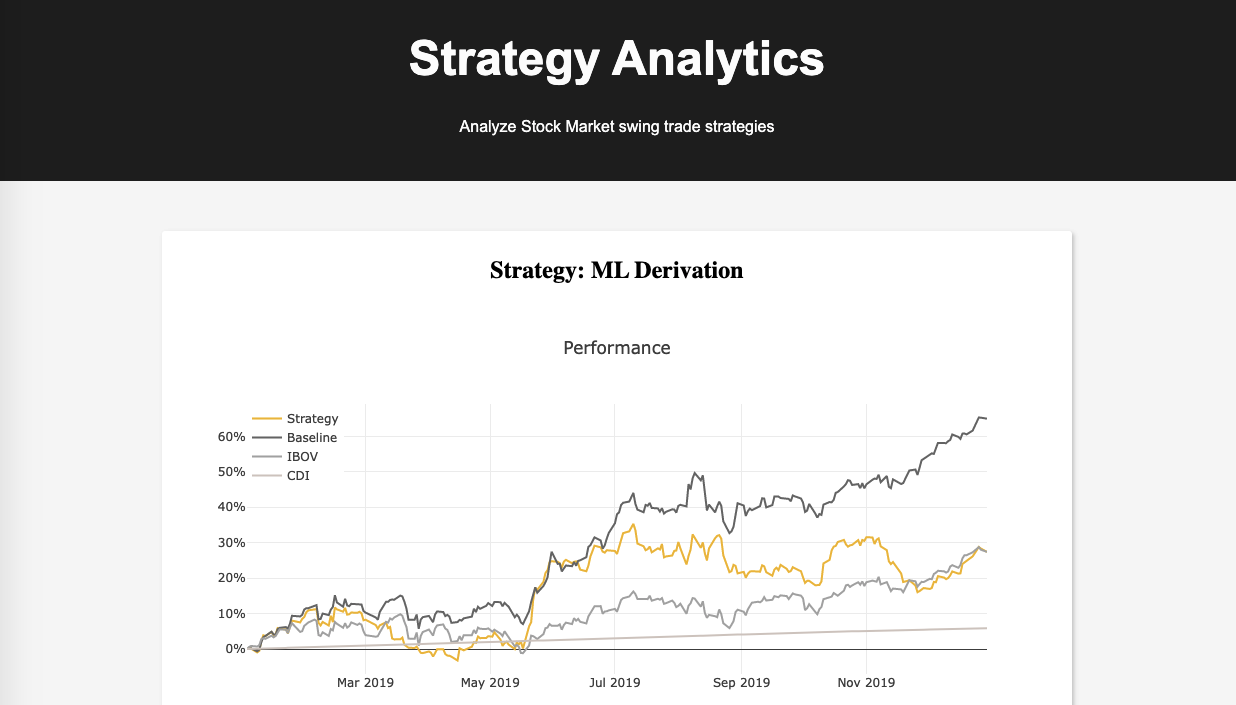
\includegraphics[scale=0.40]{dash_1.png}
    \centering
    \caption{\textit{Dashboard} - Performance}
    \label{fig:171}
\end{figure}

\begin{figure}[!htb]
    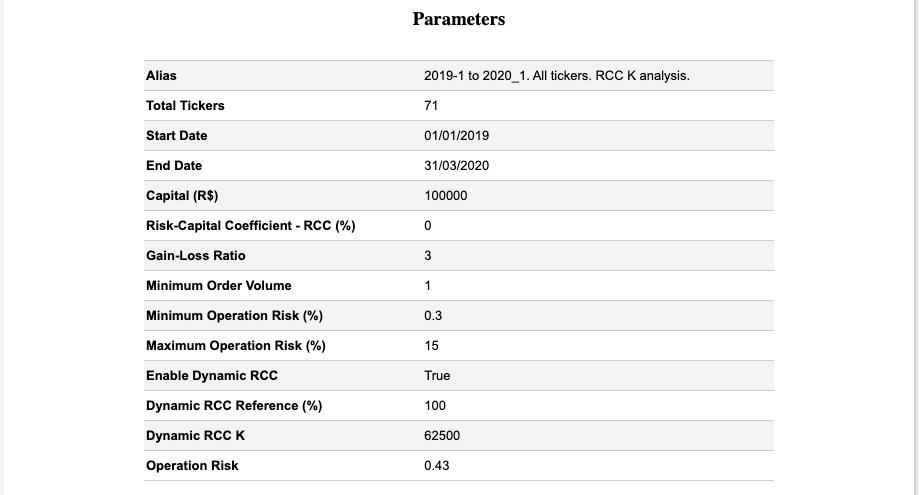
\includegraphics[scale=0.40]{dash_2.png}
    \centering
    \caption{\textit{Dashboard} - Parâmetros de entrada}
    \label{fig:172}
\end{figure}

\begin{figure}[!htb]
    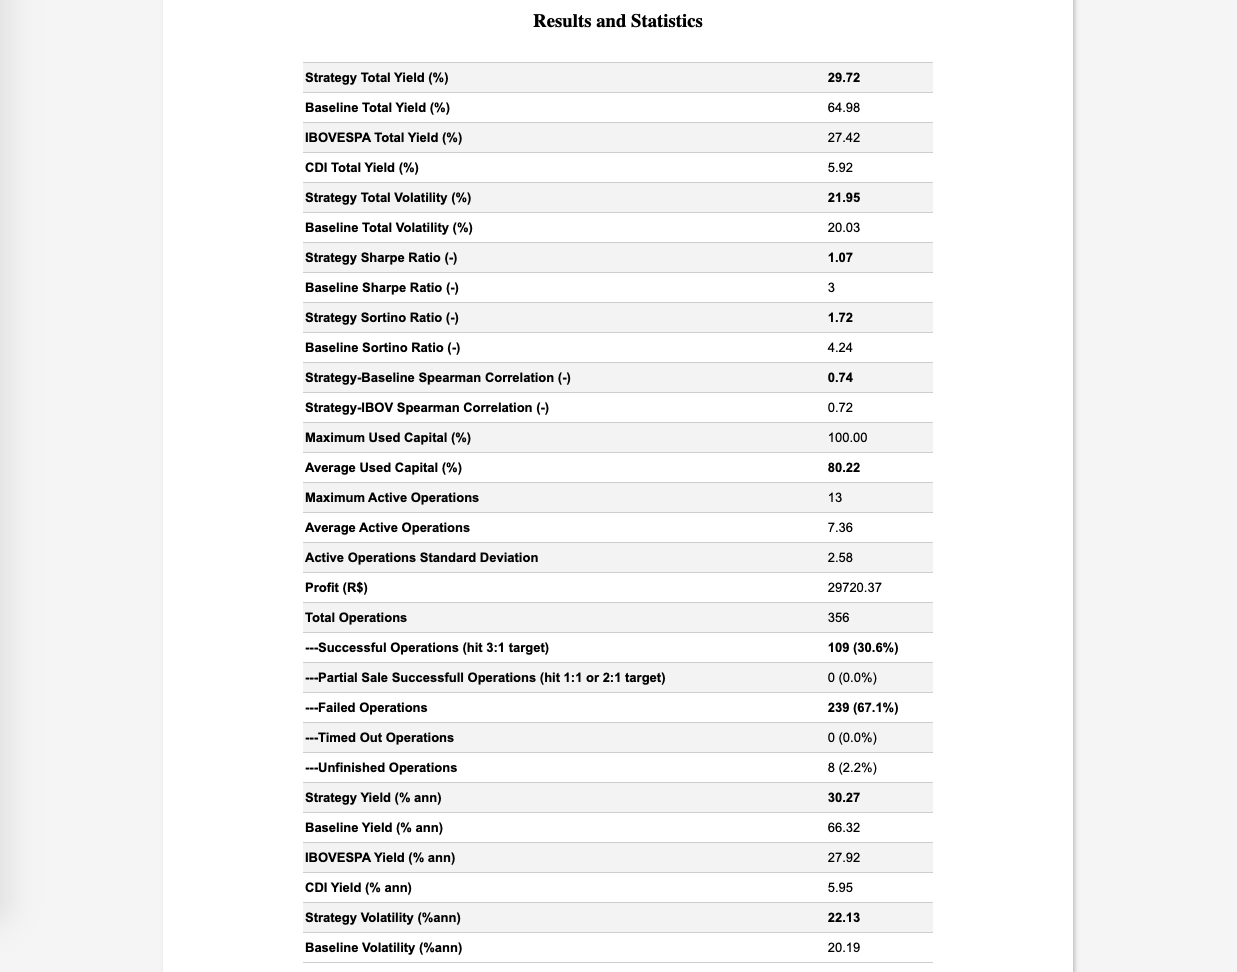
\includegraphics[scale=0.40]{dash_3.png}
    \centering
    \caption{\textit{Dashboard} - Resultados e estatísticas}
    \label{fig:173}
\end{figure}

\begin{figure}[!htb]
    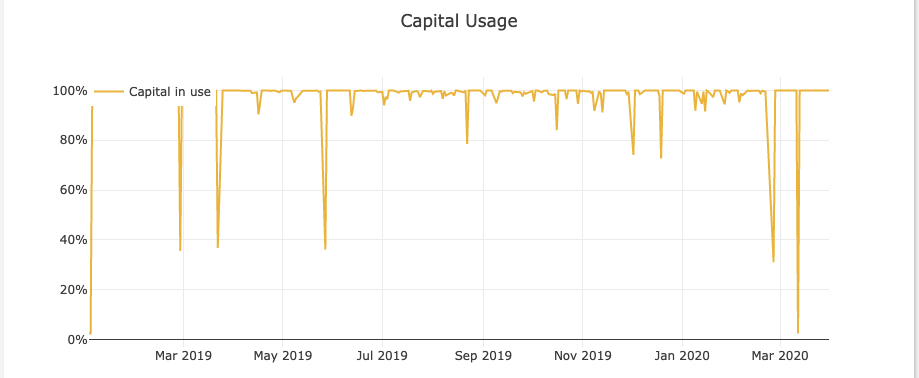
\includegraphics[scale=0.40]{dash_4.png}
    \centering
    \caption{\textit{Dashboard} - Gráfico de uso de capital}
    \label{fig:174}
\end{figure}

\begin{figure}[!htb]
    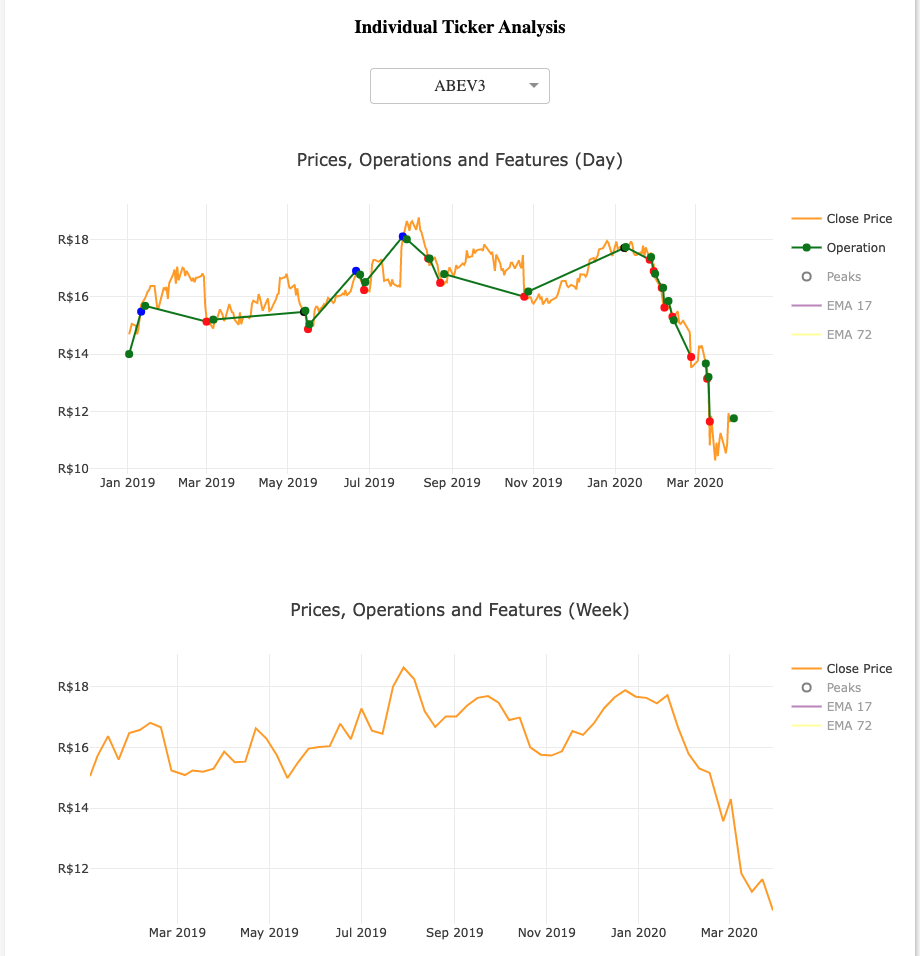
\includegraphics[scale=0.40]{dash_5.png}
    \centering
    \caption{\textit{Dashboard} - Gráficos de análise individual de ações }
    \label{fig:175}
\end{figure}



% \FloatBarrier
% \section{Otimizações de Gerenciamento de Carteira}



% \FloatBarrier
% \subsection{Resumo}

% \paragraph{} As otimizações apresentadas nesta Seção independem de um modelo de ML específico, sendo portanto algoritmos gerais que, motivados ou não por problemas oriundos dos modelos, buscam uma abordagem geral para aumento da performance da carteira.



% \subsection{Normalização por Frequência de Operações}
% \label{sub:freq_norm}

% \paragraph{} Cada ativo de uma carteira possui um critério próprio de análise das condições de mercado que o auxilia na decisão de entrada nas operações. Muitas vezes, ativos diferentes acumulam um número bastante variado de operações concluídas ao longo da simulação. O ponto esse número não posui ligação direta com a performance individual dos mesmos. Em outras palavras, facilmente ocorre a situação de um \textit{ticker} monopolizar grande parte do capital total da carteira ao longo do tempo, simplesmente por ter uma frequência de operações maior que os outros, sem qualquer fator meritocrático que embase uma justificativa.

% \paragraph{} A fim de se endereçar essa questão, foi criado o critério de Normalização por Frequência de Operações, onde cada ativo receberá de capital para uma determinada operação um valor inversamente proporcional a frequência de operações acumulada até o momento.

% \paragraph{} As Equações \ref{eq:80} e \ref{eq:81} mostram a obtenção do novo Capital Normalizado \begin{math} Capital_{norm} \end{math} a partir: do capital que em princípio seria alocado (Equação \ref{eq:61}); da frequência média de operações totais acumuladas pela carteira \begin{math} \overline{f_{total}} \end{math}; e da frequência média de operações do ativo envolvido \begin{math} f_{stock} \end{math}, igualmente acumulada.

% \begin{equation} \label{eq:80}
%     Capital_{norm} = Capital \times \dfrac{ \overline{f_{total}} }{ f_{stock}}
% \end{equation}

% \begin{equation} \label{eq:81}
%     \overline{f_{total}} = \dfrac{ N_{total\_operations} }{ N_{total\_stocks} }
% \end{equation}

% \paragraph{} Para a Normalização começar a ser aplicada a um ativo, é necessário que haja pelo menos uma operação concluída do mesmo, assim como um mínimo equivalente ao total de ativos na carteira em operações concluídas. A Equação \ref{eq:82} mostra as condições citadas.

% \begin{equation} \label{eq:82}
%     f_{stock} > 0, \quad N_{total\_operations} \ge N_{total\_stocks}
% \end{equation}

% \paragraph{} A Figura \ref{fig:130} mostra a eficácia do critério criado para a simulação dos 71 \textit{tickers} listados na Tabela \ref{tab:5}, durante o período de 01/01/2019 a 31/12/2021, onde a linha em verde denominada de \textit{benchmark} indica a ausência da Normalização e a linha em amarelo denominada por \textit{yield} indica a presença da Normalização.

% \begin{figure}[!htb] % ID: 408, 407
%     
\includegraphics[scale=0.70]{no_image.jpeg}
%     \centering
%     \caption{Simulação sem uso da Normalização por Frequência de Operações}
%     \label{fig:130}
% \end{figure}

% \begin{table}[h!]
%     \begin{center}
%         \begin{tabular}{ c|c|ccc }
%             Norm. por Freq. & Uso Médio de Cap. & Rend. Final & Sharpe & Sortino \\
%             \hline
%             Não & 68,70\% & 36,71\% & 0,4 & 0,49 \\
%             Sim & 69,23\% & 34,58\% & 0,37 & 0,44 \\
%         \end{tabular}
%         \caption{Comparação de Resultados}
%         \label{tab:6}
%     \end{center}
% \end{table}

% \paragraph{} A Figura \ref{fig:131} é análoga à Figura \ref{fig:130}, com a diferença que ambas as execuções estão com o Densanso por Tendência de Baixa e Descando por Identificação de crises ativados.

% \begin{figure}[!htb] % ID: 409, 410
%     
\includegraphics[scale=0.70]{no_image.jpeg}
%     \centering
%     \caption{Simulação com uso da Normalização por Frequência de Operações}
%     \label{fig:131}
% \end{figure}

% % \paragraph{} A Tabela \ref{tab:6} traz um comparativo dos resultados das simulações. Observa-se que o critério de Normalização criado se auto-compensa, ou seja, realoca capital dentro da própria estratégia sem grandes alterações no Uso Médio de Capital da carteira. A vantagem de um critério auto-compensado é que ele não traz uma potencial ilusão de melhora de performance, já que a comparação de resultados entre estratégias precisa ter em vista Usos Médios de Capital razoavelmente próximos entre si para que a escolha dos RCCs individuais não influencie a análise.

% % \begin{table}[h!]
% %     \begin{center}
% %         \begin{tabular}{ c|cc }
% %             & hue & hue \\
% %             \hline
% %             hue & hue & hue \\
% %             hue & hue & hue \\
% %         \end{tabular}
% %         \caption{Comparação de Resultados}
% %         \label{tab:6}
% %     \end{center}
% % \end{table}

% % \paragraph{} (Mencionar mais comentários sobre os outros parâmetros quando tiver as imagens e a tabela).



% \FloatBarrier
% \subsection{Compensação por Lucratividade}
% \label{profit_comp}

% % \paragraph{} A Compensacão por Lucratividade é um ajuste auto-compensado\footnote{Realoca capital dentro da própria estratégia sem alterar o Uso Médio de Capital da carteira} que aumenta o capital em operações de \textit{tickers} que possuem um lucro acumulado acima da média da carteira. Da mesma forma, também diminui o capital daqueles que estão com o lucro acumulado abaixo da média da carteira.
% \paragraph{} A Compensacão por Lucratividade tem por objetivo aumentar o capital em operações de \textit{tickers} que possuem um lucro acumulado acima da média da carteira, assim como diminuir o capital daqueles que estão com o lucro acumulado abaixo da média da carteira.

% \paragraph{} A Equação \ref{eq:90} mostra a primeira etapa do cálculo da Compensação, onde \begin{math} \sigma_{eq} \end{math} é o valor em unidades de desvio padrão do quanto o lucro acumulado \begin{math} p_t \end{math} do ativo está em relação à média \begin{math} \overline{P_w} \end{math} e desvio padrão \begin{math} \sigma_w \end{math} da carteira.

% \begin{equation} \label{eq:90}
%     \sigma_{eq} = \dfrac{p_t - \overline{P_w}}{\sigma_w}
% \end{equation}

% \paragraph{} Em seguida, a Equações \ref{eq:91} e \ref{eq:92} dão sequência ao cálculo criando os coeficientes das retas que serão utilizadas diretamente na Compensação através da Figura \ref{fig:140}. Nota-se que \begin{math} C_{max} \end{math} é a variação máxima positiva que a Compensação pode alcançar. \begin{math} \sigma_s \end{math} e \begin{math} \sigma_e \end{math} são limiares de \begin{math} \sigma_{eq} \end{math} que definem lugares geométricos diferentes.

% \begin{equation} \label{eq:91}
%     m_1 = \dfrac{ C_{max} }{ \sigma_e - \sigma_s }, \quad n_1 = 1 - \sigma_s m_1
% \end{equation}

% \begin{equation} \label{eq:92}
%     m_2 = \dfrac{ C_{max} }{ \sigma_e - \sigma_s }, \quad n_2 = 1 + \sigma_s m_2
% \end{equation}

% \paragraph{} Finalmente, a Equação \ref{eq:93} mostra o cálculo final, que pode ser facilmente visualizado pela Figura \ref{fig:140}.

% \begin{equation} \label{eq:93}
%     C = \begin{cases} m_1 \sigma_{eq} + n_1, & \mbox{se } \sigma_{eq} \ge \sigma_s \quad \textrm{e} \quad \sigma_{eq} \le \sigma_e \\ m_2 \sigma_{eq} + n_2, & \mbox{se } \sigma_{eq} \le - \sigma_s \quad \textrm{e} \quad \sigma_{eq} \ge - \sigma_e \\ 1 + C_{max}, & \mbox{se } \sigma_{eq} > \sigma_e \\ 1 - C_{max}, & \mbox{se } \sigma_{eq} < - \sigma_e \\ 0, & \mbox{se } |\sigma{eq}| < \sigma_s \end{cases}
% \end{equation}

% \pgfmathsetmacro{\cmax}{0.6}
% \pgfmathsetmacro{\sigs}{0.2}
% \pgfmathsetmacro{\sige}{2.0}

% \begin{figure}[!htb]
%     \centering
%     \begin{center}
%         \begin{tikzpicture}
%             \begin{axis}
%             [
%                 ylabel={Compensa\c{c}\~ao [-]},
%                 xlabel={$Lucro [\sigma_{eq}]$},
%                 xmin=-3, xmax=3,
%                 ymin=0, ymax=2,
%                 xtick={-3, -2, -1, 0, 1, 2, 3},
%                 ytick={0, 0.2, 0.4, 0.6, 0.8, 1, 1.2, 1.4, 1.6, 1.8, 2.0},
%                 ymajorgrids=true,
%                 xmajorgrids=true,
%                 grid style=dashed,
%             ]
%             \addplot[line width=0.50mm, domain=-\sigs:\sigs,blue]{1};
%             \addplot[line width=0.50mm, domain=\sigs:\sige,blue]{x * \cmax / (\sige - \sigs) + (1 - \cmax * \sigs / (\sige - \sigs))};
%             \addplot[line width=0.50mm, domain=-\sige:-\sigs,blue]{x * \cmax / (\sige - \sigs) + (1 + \cmax * \sigs / (\sige - \sigs))};
%             \addplot[line width=0.50mm, domain=\sige:10,blue]{1 + \cmax};
%             \addplot[line width=0.50mm, domain=-10:-\sige,blue]{1 - \cmax};
%             \end{axis}

%         \end{tikzpicture}
%     \end{center}
%     \caption{Gráfico da Função de Compensação por Lucratividade para \begin{math} C_{max} = 0.60\end{math}, \begin{math} \sigma_s = 0.2 \end{math} e \begin{math} \sigma_e = 2.0 \end{math}}
%     \label{fig:140}
% \end{figure}

% \paragraph{} A Figura \ref{fig:141} apresenta indicadores de performance para valores de \begin{math} C_{max} \end{math}, \begin{math} \sigma_s \end{math} e \begin{math} \sigma_e \end{math}. Foram utilizados na simulação os 71 \textit{tickers} indicados na Tabela \ref{tab:5} no intervalo de 01/01/2019 a 31/12/2021.
% O gráfico mostra que ...

% % ID:
% \begin{figure}[!htb]
%     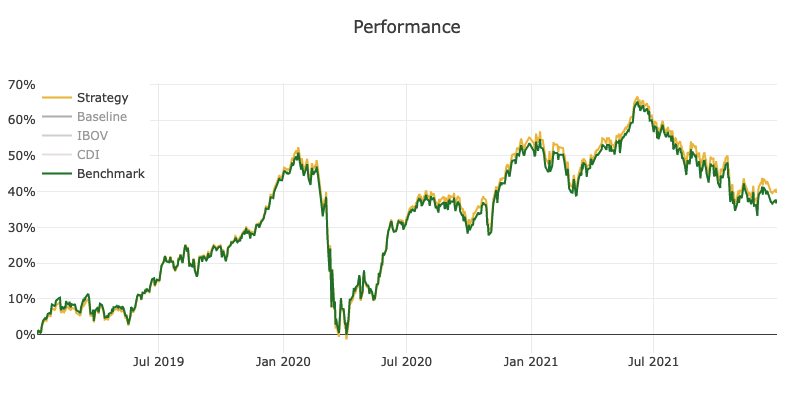
\includegraphics[scale=0.75]{profit_comp.png}
%     \centering
%     \caption{Performance por uso de Compensação por Lucratividade}
%     \label{fig:141}
% \end{figure}

% \paragraph{} Utilizou-se \begin{math} C_{max} = 0.60\end{math}, \begin{math} \sigma_s = 0.2 \end{math} e \begin{math} \sigma_e = 2.0 \end{math}.

% \paragraph{} A Figura \ref{fig:141} mostra o ganho de performance obtido para a simulação dos 71 \textit{tickers} listados na Tabela \ref{tab:5} durante o período de 01/01/2019 a 31/12/2021. A linha em amarelo indica a simulação com uso da Compensação enquanto a linha verde indica a simulação sem seu uso. Nenhuma outra otimização foi utilizada. A Tabela \ref{tab:9} traz um comparativo dos resultados das simulações. Nota-se que o RCC foi ajustado para que o Uso Médio de Capital de ambas simulações ficassem próximos.

% % ID: 415 (sem), 414 (com)
% \begin{figure}[!htb]
%     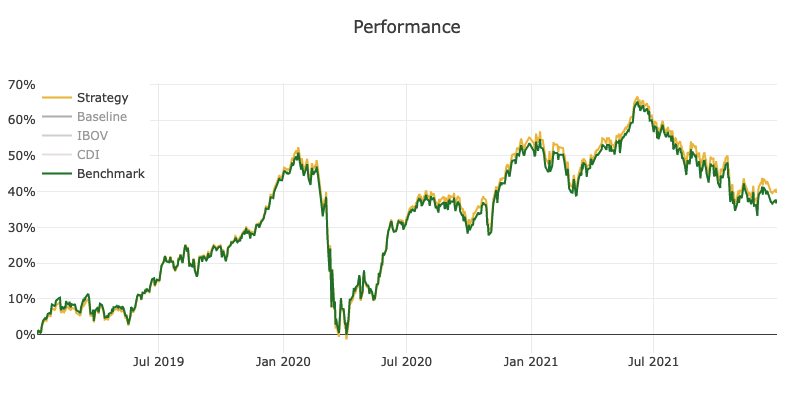
\includegraphics[scale=0.50]{profit_comp.png}
%     \centering
%     \caption{Performance por uso de Compensação por Lucratividade}
%     \label{fig:141}
% \end{figure}

% \begin{table}[h!]
%     \begin{center}
%         \begin{tabular}{ c|cc|ccc }
%             Comp. Luc. & RCC & Uso Méd. Cap. & Rend. Final & Sharpe & Sortino \\
%             \hline
%             Não & 0,35\% & 78,30\% & 42,06\% & 0,43 & 0,52 \\
%             Sim & 0,22\% & 78,74\% & 44,58\% & 0,46 & 0,55 \\
%         \end{tabular}
%         \caption{Compensação por Lucratividade - Comparação de Resultados}
%         \label{tab:9}
%     \end{center}
% \end{table}



% \FloatBarrier
% \subsection{Descanso por Tendência de Baixa}
% \label{sub:downtrend_halt}

% \paragraph{} O Descanso por Tendência de Baixa é um intervalo que impede qualquer nova operação durante a ativação do \textit{Flag} de Tendência de Baixa (ver Seção \ref{sub:features}). O objetivo é esperar o mercado entrar em uma nova tendência de alta ou pelo menos se estabilizar para que uma nova operação se justifique, mesmo que esta decisão implique em uma pequena inércia. Operações em vigor não são canceladas.

% \paragraph{} A Figura \ref{fig:152}, \ref{fig:153} e \ref{fig:154} apresentam indicadores de performance para valores de RCC e de K diferentes. Foram utilizados na simulação os 71 \textit{tickers} indicados na Tabela \ref{tab:5} no intervalo de 01/01/2019 a 31/12/2021. Cada curva

% % ID: 706
% \begin{figure}[!htb]
%     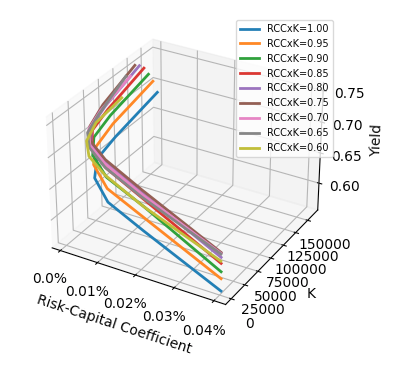
\includegraphics[scale=0.70]{yield_per_rcc_k.png}
%     \centering
%     \caption{Rendimento sob uso de RCC dinâmico}
%     \label{fig:160}
% \end{figure}




% \FloatBarrier
% \subsection{Descanso por Identificação de Crises}
% \label{sub:crisis_halt}

% \paragraph{} O Descanso por Identificação de Crises é um intervalo que impede qualquer nova operação durante a ativação do \textit{Flag} de Identificação de Crises (ver Seção \ref{sub:features}). O objetivo é esperar o mercado se estabilizar de uma crise em potencial para que uma nova operação se justifique, mesmo que esta decisão implique em uma pequena inércia. Operações em vigor não são canceladas. \color{red} HERALDO: Optei por não colocar uma imagem mostrando a eficácia desse flag porque em princípio a Seção de Features (\ref{sub:features}) já faz isso. \color{black}






% \begin{math} R_b \end{math}
% \color{red} HERALDO: \colorend
% \color{red} HERALDO: \color{black}